\documentclass[11pt,a4paper]{article}
\usepackage[margin=25mm,headheight=14pt,headsep=8mm]{geometry}
\usepackage{fontspec}
\IfFontExistsTF{Liberation Serif}{%
  \setmainfont{Liberation Serif}%
}{%
  \setmainfont{Times New Roman}%
}
\IfFontExistsTF{Liberation Sans}{%
  \setsansfont{Liberation Sans}%
}{%
  \setsansfont[Path=../../../../../tools/books/.cache/fonts/,
    BoldFont=DejaVuSans-Bold.ttf,
    ItalicFont=DejaVuSans-Oblique.ttf,
    BoldItalicFont=DejaVuSans-BoldOblique.ttf]{DejaVuSans.ttf}%
}
\IfFontExistsTF{DejaVu Sans Mono}{%
  \setmonofont[Scale=0.86]{DejaVu Sans Mono}%
}{%
  \setmonofont[Path=../../../../../tools/books/.cache/fonts/,
    Scale=0.86,
    BoldFont=DejaVuSansMono-Bold.ttf,
    ItalicFont=DejaVuSansMono-Oblique.ttf,
    BoldItalicFont=DejaVuSansMono-BoldOblique.ttf]{DejaVuSansMono.ttf}%
}
\usepackage{amsmath,amssymb,amsthm}
\usepackage{microtype}
\usepackage{setspace}
\setstretch{1.15}
\usepackage{longtable,booktabs,array,calc}
\newcounter{none}
\usepackage{needspace}
\usepackage{graphicx}
\usepackage{fancyhdr}
\usepackage[authoryear,round]{natbib}
\usepackage{xcolor}
\definecolor{linkblue}{HTML}{004B87}
\PassOptionsToPackage{hyphens}{url}
\usepackage[unicode,colorlinks=true,allcolors=linkblue,bookmarksnumbered=true]{hyperref}
\usepackage{xurl}
\urlstyle{same}
\hypersetup{
  pdftitle={Prepayment Thresholds, Informative Zero Receipts, and
Certified Polynomial Decision Diagrams in Partially Observed
Regenerative Maintenance},
  pdfauthor={},
  pdfsubject={Mathematics of Operations Research Blinded Manuscript},
  pdfkeywords={Bayesian dynamic programming; partially observable Markov
decision processes; regenerative maintenance and standby control;
sufficient statistics and decision diagrams; certifying algorithms}
}
\setlength{\parindent}{1.15em}
\setlength{\parskip}{2pt}
\setlength{\emergencystretch}{3.5em}
\setcounter{secnumdepth}{2}
\widowpenalty=10000
\clubpenalty=10000
\displaywidowpenalty=10000
\providecommand{\tightlist}{\setlength{\itemsep}{2pt}\setlength{\parskip}{0pt}}
\providecommand{\passthrough}[1]{#1}
\pagestyle{fancy}
\fancyhf{}
\fancyhead[L]{\footnotesize Prepayment Thresholds and Certified Polynomial Decision Diagrams}
\fancyhead[R]{\footnotesize Mathematics of Operations Research (Blinded Submission)}
\fancyfoot[C]{\small\thepage}
\renewcommand{\headrulewidth}{0.25pt}
\fancypagestyle{plain}{\fancyhf{}\fancyfoot[C]{\small\thepage}\renewcommand{\headrulewidth}{0pt}}
\begin{document}
\thispagestyle{plain}
\begin{flushleft}
{\fontsize{17.5}{22}\selectfont\bfseries Prepayment Thresholds,
Informative Zero Receipts, and Certified Polynomial Decision Diagrams in
Partially Observed Regenerative Maintenance\par}
\vspace{8pt}
{\small\emph{Blinded manuscript prepared for double-anonymous review at Mathematics of Operations Research}\par}
\end{flushleft}
\vspace{6pt}
\hrule height 0.4pt
\vspace{8pt}
\noindent\textbf{Abstract.}\quad Maintaining a regenerative standby
system under partial observation and a non-replenished operational
budget requires deciding jointly when to pay for active repair, which
redundant unit to dispatch, and when to halt paid intervention. Unlike
average-cost constrained models or memoryless adaptive control, we study
a persistent unknown operating reliability drawn once from a finite
prior, where every repair request must satisfy hard sample-path
prepayment before its uncertain outcome is observed and the controller
receives only coarse two-bit post-transaction receipts recording
reproduction and actual fee deduction. Within a self-contained
mathematical framework accompanied by a pure-kernel machine-checked
formalization, we establish exact commutation between the complete
genealogical population process and a compressed belief-and-wallet
dynamic program achieving Bayes optimality over all real-randomized
history policies. In the single-repair high-price regime, we derive a
closed-form optimal value formula, sharp positivity thresholds, strict
post-fault posterior threshold contraction, positive receipt-feedback
gain, and zero post-repair value of parameter revelation. Finally, by
separating informative fault receipts from deterministic zero receipts,
we prove joint all-action sufficiency of a five-coordinate counting
summary and verify an all-action certifying decision-diagram synthesizer
satisfying an explicit quartic node bound.\par
\vspace{6pt}
\noindent{\small\textbf{Keywords:}\quad Bayesian dynamic programming;
partially observable Markov decision processes; regenerative maintenance
and standby control; sufficient statistics and decision diagrams;
certifying algorithms}\par
\vspace{3pt}
\noindent{\small\textbf{MSC 2020 Subject Classification:}\quad Primary:
90C40, 93E20; Secondary: 60J85, 62C10, 68V15}\par
\vspace{3pt}
\noindent{\small\textbf{OR/MS Subject Classification:}\quad Dynamic
programming/optimal control: Markov, Bayesian; Probability: branching
processes; Reliability: maintenance/repairs}\par
\vspace{8pt}
\hrule height 0.4pt
\vspace{12pt}

\section{Introduction: adaptive standby maintenance under hard
prepayment and coarse
receipts}\label{introduction-adaptive-standby-maintenance-under-hard-prepayment-and-coarse-receipts}

Sequential maintenance and standby dispatch in regenerative stochastic
systems sit at the intersection of three classical streams in operations
research: controlled branching and reliability theory
\citep{harris1963, sevastyanov1971, athreyaNey1972, barlowProschan1975, pliska1976, rothblumWhittle1982},
Bayesian adaptive dynamic programming under incomplete state and
parameter information
\citep{bellman1957, bellman1961, astrom1965, rieder1975, bertsekasShreve1978, easleyKiefer1988},
and state-space or policy-graph compression via sufficient statistics
and decision diagrams
\citep{striebel1965, dynkin1978, bryant1986, boutilier2000, bergman2016}.
Consider an operator managing a fault-prone regenerative service or
biological lineage initialized with a single damaged primary unit
(\texttt{root0}). At each discrete decision epoch
\(t \in \{0, \dots, H-1\}\), the operator may either permanently commit
to passive operation (\texttt{stop}), dispatch the primary unit or a
spawned standby unit (\texttt{child1}) without intervention
(\texttt{idle}), or submit a paid active repair request
(\texttt{write}). Under normal operation---occurring at each step with a
\emph{persistent unknown reliability}
\(r_\theta \in [0,1] \cap \mathbb{Q}\) governed by a latent environment
parameter \(\theta \sim \pi_0\) drawn once at initialization---an intact
or repaired unit produces one unit of reproductive or service output
(spawning a healthy standby unit at \texttt{child1} upon the first
successful birth) and, if a repair was requested, incurs a fixed fee
\(c > 0\). Under a runtime fault---occurring with probability
\(1 - r_\theta\)---the dispatched unit is left damaged, no output is
produced, and no write fee is charged.

Despite its compact physical specification, solving and certifying exact
finite-horizon optimal control for such a system exposes four structural
phenomena that standard Markov decision process (MDP) and partially
observable Markov decision process (POMDP) treatments routinely separate
or idealize away:

\begin{enumerate}
\def\labelenumi{\arabic{enumi}.}
\tightlist
\item
  \emph{Hard sample-path prepayment versus average budget constraints.}
  Classical constrained MDPs \citep{altman1999, feinberg2000} constrain
  expected cumulative expenditure \(\mathbb{E}[\sum_t C_t] \le B_0\),
  permitting individual sample paths to overdraw the budget provided
  other paths compensate. Even hard-budget sequential allocation models
  such as bandits with knapsacks
  \citep{badanidiyuru2018, besbesZeevi2009} typically deduct
  deterministic or post-realization costs without coupling pre-execution
  collateral to fault-contingent billing. In physical escrow, autonomous
  spacecraft, or metabolic energy allocation, by contrast, submitting a
  repair request requires holding literal balance \(B_t \ge c\)
  \emph{prior to execution} on \emph{every positive-probability
  trajectory}, even though a subsequent runtime fault or empty standby
  slot leaves ex-post charge \(C_t = 0\). Consequently, average
  expenditure never substitutes for pathwise liquidity, and an initial
  balance \(B_0 < c\) enforces strict zero-value impossibility across
  arbitrarily long horizons even when repairs would be profitable in
  expectation.
\item
  \emph{Coarse post-transaction receipts hiding native genealogical
  worlds.} Inspection and replacement models under partial observation
  \citep{eckles1968, ross1970, ross1971, white1979, monahan1982, makisJiang2003}
  typically model a single deteriorating machine without population
  growth. Conversely, multitype controlled branching models
  \citep{jagers1975, pliska1976, rothblumWhittle1982, haccou2005, gonzalez2018}
  typically observe complete population census vectors. Here, the
  underlying native population store \(\mathcal{S}_t\) grows by one slot
  per transaction---recording parent--offspring lineages, individual
  clocks, fair birth labels, and failed-birth \texttt{None} markers
  across unbounded addresses \(j \ge 0\)---yet the controller observes
  \emph{only} its own requested actions and a two-bit post-transaction
  receipt \(o_t = (\mathrm{birth}_t, \mathrm{paid}_t) \in \{0,1\}^2\).
  Proving that a finite-memory receipt controller achieves exact Bayes
  optimality in the \emph{native genealogical world} requires an
  explicit measure-preserving commutation bridge rather than merely
  defining a reduced POMDP by fiat.
\item
  \emph{Non-myopic high-price thresholds, persistent variance premiums,
  and subtle value of information.} When the priced repair fee
  \(p = \lambda c\) exceeds single-step output (\(p > 1\)), any myopic
  one-step controller refuses repair and earns zero. Over a multi-step
  horizon \(H+1\), however, a single successful initial repair
  simultaneously restores \texttt{root0} and populates the standby unit
  \texttt{child1}, unlocking a zero-fee receipt-switching continuation
  that hedges subsequent faults across two bodies. Simultaneously,
  because \(\theta\) is drawn \emph{once} and persists across all
  \(H+1\) steps
  \citep{wald1947, raiffaSchlaifer1961, martin1967, degroot1970},
  multi-step payoffs depend on higher prior moments
  \(\mu_k = \mathbb{E}[r_\theta^k]\) rather than powers of the mean
  \(\mu_1^k\). After an uncharged initial fault receipt \((0,0)\),
  Bayesian updating shifts posterior weight toward lower reliability
  \citep{aghion1991, duff2002, ross2011, ghavamzadeh2015}, contracting
  the retry profitability threshold. Yet once a repair succeeds and
  exhausts a unit wallet \(B_0 = c\), does additional information about
  \(\theta\) retain positive value \citep{blackwell1953, howard1966}? As
  we prove, adaptive switching based on \emph{body-status receipts}
  yields strictly positive feedback value at \(H+1 \ge 4\), whereas
  revealing the true parameter \(\theta\) \emph{for free} after wallet
  exhaustion yields \emph{exact zero additional value}.
\item
  \emph{Informative versus uninformative zero receipts and all-action
  certified decision diagrams.} Over horizon \(H\) with
  \(|\mathcal{A}| = 7\) actions and \(|\mathcal{O}| = 4\) receipts, an
  uncompressed history-table representation branches at rate
  \((|\mathcal{A}||\mathcal{O}|)^H = 28^H\)
  (\(28^8 \approx 3.78 \times 10^{11}\) at \(H=8\))
  \citep{papadimitriouTsitsiklis1987, lovejoy1991, cassandra1997, kaelbling1998, madani2003}.
  Compressing this tree into a shared directed acyclic decision diagram
  \citep{bryant1986, bahar1997, hoey1999, hansen1998, meuleau1999, poupartBoutilier2003}
  without losing exact optimality over arbitrary real-randomized history
  policies requires identifying an exact sufficient statistic
  \citep{halmosSavage1949, striebel1965, hinderer1970, subramanian2022}.
  Crucially, \emph{not every \((0,0)\) receipt is a statistical fault
  sample}: idling an already-damaged unit or addressing a non-existent
  standby slot produces \((0,0)\) with conditional probability \(1\)
  under \emph{every} reliability \(r_\theta\), so treating all zero
  receipts symmetrically corrupts the Bayesian posterior. Furthermore,
  following the paradigm of certifying algorithms
  \citep{blumKannan1995, mcconnell2011} and interactive theorem proving
  \citep{nipkowPaulsonWenzel2002, bertotCasteran2004, hoelzl2017, mouraUllrich2021, schaeffelerAbdulaziz2023},
  a shared policy graph cannot certify global optimality merely by
  checking the reachable optimal subgraph: omitting a
  positive-probability branch of even an \emph{unselected} suboptimal
  action invalidates the Bellman upper bound.
\end{enumerate}

\subsubsection{Summary of main
contributions}\label{summary-of-main-contributions}

This article resolves all four problems within a completely
self-contained mathematical development accompanied by an end-to-end
pure-kernel formalization in the Lean 4 theorem prover
\citep{mouraUllrich2021, mathlib2020} depending exclusively on Lean's
three foundational logical axioms (\texttt{propext},
\texttt{Classical.choice}, \texttt{Quot.sound}; \citet{carneiro2019}),
with zero incomplete proofs (\texttt{sorryAx}) and zero compiler-trust
evaluation axioms (\texttt{native\_decide} / \texttt{Lean.ofReduceBool};
\citet{boespflug2011}; \citet{boutin1997}). Every mathematical theorem,
closed-form recursion, posterior moment inequality, history-separation
witness, and polynomial graph bound is proved in full in the
Mathematical Appendix so that the paper can be read and refereed
entirely as a standalone work in stochastic operations research. Our six
main theorems establish:

\begin{itemize}
\tightlist
\item
  \textbf{Native-to-compressed commutation, pathwise prepayment, and
  full-history Bayes optimality (Section 2, Theorem 1).} Under inherited
  target alignment (\texttt{Aligned}), we prove exact step-by-step
  commutation between the native genealogical population store
  \(\mathcal{S}_t\) and a compressed optional-bit store over arbitrary
  primitive mode-and-label sequences. Constructing the joint
  belief--wallet dynamic program over \((b_t, B_t)\), we prove that the
  computably returned finite policy table satisfies strict pre-execution
  prepayment \(0 \le C_t \le c\,\mathrm{cap}(a_t) \le B_t\) on every
  positive-probability prefix and achieves exact Bayes optimality across
  \emph{all} causal strategies employing arbitrary real randomization
  weights over complete permitted action--receipt histories
  (\texttt{SupportedAdmissible}), without imposing artificial legality
  constraints on zero-probability counterfactual branches.
\item
  \textbf{Exact high-price closed-form value, two-object backup
  recursion, and sharp positivity threshold (Section 3, Theorem 2).} For
  horizon \(H+1\), single-repair wallet \(B_0 = c\), priced write fee
  \(p = \lambda c\), and discount sum \(S_H(d) = \sum_{t=0}^{H-1} d^t\),
  we derive the exact zero-write one-unit and two-unit continuation
  recursions \(U_1(r,d,n)\) and \(U_2(r,d,n)\) attained by
  receipt-driven standby switching (\texttt{freeSchedule}). Whenever
  \(p \ge S_H(d)\), we prove the exact closed-form Bayes-optimal value
  \[V_{H+1}^* = \max\Bigl\{0,\ \mathbb{E}_{\pi_0}\bigl[r_\theta\bigl(1 - p + d\, U_2(r_\theta, d, H)\bigr)\bigr]\Bigr\},\]
  yielding the sharp necessary-and-sufficient positivity criterion
  \(V_{H+1}^* > 0 \iff p < 1 + d\,\mathbb{E}[r_\theta U_2(r_\theta, d, H)] / \mathbb{E}[r_\theta]\),
  alongside universal pathwise zero-value impossibility \(V_H^* = 0\)
  whenever \(B_0 < c\).
\item
  \textbf{Persistence variance premium, post-fault threshold drop,
  receipt-feedback gain, and zero post-repair value of
  \(\theta\)-revelation (Section 4, Theorem 3).} Specializing to short
  horizons and general priors, we prove: (i) persistent \(\theta\)
  exceeds i.i.d. step-redrawn \(\theta\) on the two-step repair
  candidate by exact margin \(d\,\mathrm{Var}(r_\theta) \ge 0\)
  (\(+1/160\) vs.~\(-1/40\)); (ii) for any nondegenerate two-point prior
  \(0 < r_0 < r_1 < 1\) and \(d > 0\), an uncharged fault receipt
  \((0,0)\) strictly contracts the remaining two-step repair threshold
  via \(\mu_1\mu_3 - \mu_2^2 = w(1-w)r_0 r_1(r_0 - r_1)^2 > 0\)
  (\(21/16 \to 5/4\), penalizing prior-freezing retries by \(3/640\) at
  \(H=3\)); (iii) at \(H+1 = 4\), receipt-adaptive standby switching
  beats \emph{every} open-loop request sequence by raw margin
  \(d^3 \mathbb{E}[r_\theta^3(1 - r_\theta)]\) (\(20925/524288\) at
  \(r \in \{3/4, 7/8\}\)); yet (iv) once initial repair succeeds and
  exhausts the wallet, \texttt{freeSchedule} attains the
  \(\theta\)-omniscient upper bound simultaneously for all
  \(r \in [0,1]\), rendering post-repair \(\theta\)-revelation strictly
  worthless (\(\mathrm{EVPI}_{\mathrm{post}} = 0\)).
\item
  \textbf{Informative zero-receipt filtering and universal
  counting-posterior factorization (Section 5.1, Theorem 4).}
  Characterizing informative step configurations via
  \(\mathrm{informative}(g, q, a) \iff o_{\mathrm{norm}}(g, q, a) \neq (0,0)\),
  we prove that for \emph{every} causal real-randomized full-history
  strategy \(\pi\) and \emph{every} positive-mass history \(h\), the
  strategy's pathwise randomization factor \(\alpha_\pi(h) > 0\) is
  \(\theta\)-independent and cancels identically, reducing the exact
  posterior to
  \(\pi_h(\theta) = \pi_0(\theta) r_\theta^{s(h)}(1 - r_\theta)^{f(h)} / Z(s(h), f(h))\)
  including endpoint rates \(r_\theta \in \{0,1\}\) (\(0^0 = 1\)) and
  zero-prior atoms.
\item
  \textbf{Joint all-action sufficiency of \(\sigma = (t, q, s, f, k)\)
  and three-way sharpness separations (Section 5.2, Theorem 5).} We
  prove that the five-coordinate operational summary
  \(\sigma = (t, q, s, f, k)\) (with \(|Q| = 24\), \(n + t = H\), and
  literal wallet \(B_0 - kc\)) preserves feasible action menus and the
  \emph{joint} single-step distribution over receipt, next summary,
  birth, literal fee, and next wallet for \emph{every} legal action.
  Conversely, explicit reachable witnesses prove that: (a) the physical
  Markov triple \((t, q, B)\) is \emph{insufficient} (\(5/8 \neq 1/2\)
  next-birth probability); (b) distinct native histories with
  non-isomorphic genealogical tail stores
  (\([\neg g, g, \mathrm{None}, g] \neq [\neg g, g, g, \mathrm{None}]\))
  \emph{lawfully merge} to a single shared node; and (c) enlarging
  future dispatch permissions to \texttt{address\ 2} immediately breaks
  that merger (\(0\) vs.~\(r_\theta\)).
\item
  \textbf{All-action certifying decision diagrams and explicit quartic
  node bound \(N_H \le 24(H+1)^4\) (Section 6, Theorem 6).} Decoupling
  untrusted memoized graph generation (\texttt{generate}) from an
  executable rational certificate checker
  (\texttt{certify\ :\ Option\ Certified}), we prove that every accepted
  shared array \texttt{Graph} achieves exact native full-history Bayes
  optimality, satisfies pathwise literal prepayment, rejects omitted
  unselected-action successors, and obeys the certified size bound
  \(N_H = \mathrm{Graph.size} \le 24(H+1)^4\)---compressing
  \(28^8 \approx 3.78 \times 10^{11}\) raw branches at \(H=8, B_0=2\)
  into \(1,661\) certified all-action nodes and \(151\) optimal
  execution nodes with exact optimal value \(884450457 / 1342177280\).
\end{itemize}

\section{Native population semantics, sample-path prepayment, and
full-history Bayes
optimality}\label{native-population-semantics-sample-path-prepayment-and-full-history-bayes-optimality}

\subsection{Genealogical population store, seven-action menu, and
pre-execution fee
commitment}\label{genealogical-population-store-seven-action-menu-and-pre-execution-fee-commitment}

Let \(g \in \{0,1\}\) denote a publicly known operational target bit
(without loss of generality, \(g = 1\) in concrete benchmarks). An
environment parameter \(\theta\) is drawn once at initialization
\(t = 0\) from a finite prior probability mass function
\(\pi_0 \in \Delta(\Theta)\), where each \(\theta \in \Theta\) specifies
a persistent rational normal-mode reliability
\(r_\theta \in [0,1] \cap \mathbb{Q}\)
\citep{wald1950, savage1954, rieder1975}. Conditional on \(\theta\), the
environment generates at each discrete step \(t \in \{0, \dots, H-1\}\)
an independent primitive noise pair
\(z_t = (m_t, \ell_t) \in \{0,1\}^2\), where \(m_t \in \{0,1\}\)
indicates normal execution (\(m_t = 1\) with probability \(r_\theta\))
versus runtime fault (\(m_t = 0\) with probability \(1 - r_\theta\)),
and \(\ell_t \in \{0,1\}\) is an independent fair birth-lineage label
(\(\mathbb{P}(\ell_t = 1) = 1/2\)) so that the joint single-step
primitive weight is
\[K_\theta(m, \ell) := \frac{1}{2}\bigl(r_\theta \mathbf{1}_{\{m=1\}} + (1 - r_\theta)\mathbf{1}_{\{m=0\}}\bigr) \in \mathbb{Q}_{\ge 0}, \qquad \sum_{(m,\ell) \in \{0,1\}^2} K_\theta(m, \ell) = 1.\]

In the underlying \emph{native genealogical world}, the population at
step \(t\) is an append-only indexed store
\(\mathcal{S}_t = [\xi_0, \xi_1, \dots, \xi_{L_t - 1}]\) of length
\(L_t = 1 + t\), where each slot \(\xi_j\) holds either \texttt{None}
(recording a transaction that produced no offspring) or
\texttt{Some}\(\,(p_j)\) for a clocked individual \(p_j\) carrying: (i)
its mutable physical state bit \(x_j \in \{0,1\}\); (ii) an immutable
inherited program bit \(\mathrm{prog}(p_j) \in \{0,1\}\); (iii) its
immutable genealogical identity chain recording ancestor slot indices
and fair birth labels \(\ell\); and (iv) its individual age clock
incremented whenever slot \(j\) is dispatched
\citep{jagers1975, haccou2005}. Crucially, undispatched slots retain
their physical bits and clocks unchanged---the population does
\emph{not} undergo simultaneous global aging. Initialization starts from
a single damaged founder at slot \(0\) whose inherited program aligns
with \(g\): \(\mathcal{S}_0 = [\mathrm{Some}(p_0)]\) with
\(x_0 = \neg g\) and \(\mathrm{prog}(p_0) = g\).

At each step \(t\), the controller selects a request \(a_t\) from a
fixed public seven-action menu \(\mathcal{A}\) ordered canonically for
deterministic tie-breaking \citep{derman1970, puterman1994}:
\[\mathcal{A} := \bigl[\mathrm{stop},\ (0, \mathrm{idle}),\ (1, \mathrm{idle}),\ (0, \mathrm{write}_0),\ (0, \mathrm{write}_1),\ (1, \mathrm{write}_0),\ (1, \mathrm{write}_1)\bigr].\]
Here address \(0\) refers to the founder slot (\texttt{root0}), address
\(1\) refers to the first post-initialization slot (\texttt{child1}),
and slots \(j \ge 2\) remain in the native population store
\(\mathcal{S}_t\) without entering the controller's dispatch menu.
Selecting \(\mathrm{stop}\) permanently sets a latched boolean flag
\(\mathrm{stopped}_{t+1} = 1\), committing the current step and
\emph{all} remaining steps \(s \ge t\) to the effective request
\((0, \mathrm{idle})\)---stopping paid intervention without freezing the
environment, subsequent births from \texttt{root0}, or native record
allocation. Formally, given current latch
\(\mathrm{stopped} \in \{0,1\}\) and nominal action
\(a \in \mathcal{A}\), the effective slot-action pair
\((j_{\mathrm{eff}}, \alpha_{\mathrm{eff}}) = \mathrm{eff}(\mathrm{stopped}, a)\)
equals \((0, \mathrm{idle})\) if \(\mathrm{stopped} = 1\) or
\(a = \mathrm{stop}\), and equals \((j, \alpha)\) if
\(\mathrm{stopped} = 0\) and \(a = (j, \alpha)\).

Executing \((j_{\mathrm{eff}}, \alpha_{\mathrm{eff}})\) on
\(\mathcal{S}_t\) under primitive realization \(z_t = (m_t, \ell_t)\)
proceeds as follows:

\begin{enumerate}
\def\labelenumi{\arabic{enumi}.}
\tightlist
\item
  \textbf{Empty-slot lookup.} If \(\mathcal{S}_t[j_{\mathrm{eff}}]\) is
  out of bounds (at \(t = 0\) when \(j_{\mathrm{eff}} = 1\)) or holds
  \texttt{None} (when the \(t=0\) transaction produced no child so slot
  \(1\) is permanently \texttt{None}), no state bit changes,
  \texttt{None} is appended at slot \(L_t\), no birth occurs, and no fee
  is charged: the delivered two-bit receipt is \(o_t = (0, 0)\) and
  literal fee is \(C_t = 0\).
\item
  \textbf{Existing-slot execution.} If
  \(\mathcal{S}_t[j_{\mathrm{eff}}] = \mathrm{Some}(p)\) with current
  physical bit \(x\) and aligned program \(\mathrm{prog}(p) = g\), let
  the candidate post-action bit under normal mode be
  \(x_{\mathrm{cand}}(x, \alpha_{\mathrm{eff}}) := x\) if
  \(\alpha_{\mathrm{eff}} = \mathrm{idle}\) and \(v\) if
  \(\alpha_{\mathrm{eff}} = \mathrm{write}_v\). Then the updated
  physical bit at slot \(j_{\mathrm{eff}}\) is
  \[x' = \mathrm{postBit}(g, x, \alpha_{\mathrm{eff}}, m_t) := \begin{cases} x_{\mathrm{cand}}(x, \alpha_{\mathrm{eff}}), & m_t = 1, \\ \neg g, & m_t = 0. \end{cases}\]
  A newborn individual with physical bit \(g\), inherited program \(g\),
  clock \(0\), and updated genealogical tag \((L_t, \ell_t)\) is
  appended at slot \(L_t\) (\(\mathrm{birth}_t = 1\)) if and only if
  \(m_t = 1\) and \(x_{\mathrm{cand}}(x, \alpha_{\mathrm{eff}}) = g\);
  otherwise \texttt{None} is appended (\(\mathrm{birth}_t = 0\)).
  Simultaneously, the literal write fee
  \(C_t = c \cdot \mathrm{paid}_t\) is charged (\(\mathrm{paid}_t = 1\))
  if and only if \(m_t = 1\) and
  \(\alpha_{\mathrm{eff}} \in \{\mathrm{write}_0, \mathrm{write}_1\}\);
  under a fault (\(m_t = 0\)) or \texttt{idle}, \(\mathrm{paid}_t = 0\)
  and \(C_t = 0\).
\end{enumerate}

The controller observes \emph{only} its own past actions and the
delivered two-bit receipts
\(o_t = (\mathrm{birth}_t, \mathrm{paid}_t) \in \mathcal{O} := \{0,1\}^2\),
never \(m_t\), \(\ell_t\), \(\theta\), or \(\mathcal{S}_t\)
\citep{astrom1965, smallwoodSondik1973, krishnamurthy2016}. A single
initial wallet \(B_0 \in \mathbb{Q}_{\ge 0}\) receives zero external
income or replenishment. Crucially, define the \emph{pre-execution write
commitment} \(\mathrm{cap}: \mathcal{A} \to \{0,1\}\) by setting
\(\mathrm{cap}(a) := 1\) for the four nominal write requests
\((j, \mathrm{write}_v)\) and \(\mathrm{cap}(a) := 0\) for
\(\mathrm{stop}\), \((0, \mathrm{idle})\), and \((1, \mathrm{idle})\).
Notice that \(\mathrm{cap}(a)\) is evaluated on the \emph{nominal}
action \(a\) independent of \(\mathrm{stopped}\), so entering the
stopped latch never unlocks nominal write labels without balance. At
wallet balance \(B_t \ge 0\), the feasible action menu is
\[\mathrm{menu}(c, B_t) := \bigl\{a \in \mathcal{A} : c\,\mathrm{cap}(a) \le B_t\bigr\},\]
which is always nonempty because
\(\mathrm{stop} \in \mathrm{menu}(c, B_t)\) for every \(B_t \ge 0\).
Because \(\mathrm{paid}_t \le \mathrm{cap}(a_t)\) holds identically
across all worlds and noise realizations, every legal request satisfies
\(0 \le C_t \le c\,\mathrm{cap}(a_t) \le B_t\), updating the wallet
deterministically from the public receipt bit via
\(B_{t+1} = B_t - c\,\mathrm{paid}_t\). Over horizon
\(H \in \mathbb{N}\) with discount factor
\(d \in [0,1] \cap \mathbb{Q}\), tariff \(c \in \mathbb{Q}_{>0}\), unit
fee price \(\lambda \in \mathbb{Q}_{\ge 0}\), and zero terminal salvage
value, any policy \(\pi\) is evaluated by its expected discounted net
output
\[J_H(\pi) := \mathbb{E}_{\pi_0, \pi}\!\left[\sum_{t=0}^{H-1} d^t \bigl(\mathrm{birth}_t - \lambda C_t\bigr)\right].\]

\subsection{Inherited-target projection and optimality over
real-randomized history
strategies}\label{inherited-target-projection-and-optimality-over-real-randomized-history-strategies}

To solve for \(J_H(\pi)\) without tracking unbounded genealogical
metadata inside the Bellman state, define the \emph{compressed world}
\(w = (\theta, s, \mathrm{stopped}) \in \mathcal{W}(\Theta)\), where
\(\mathcal{W}(\Theta) := \Theta \times (\mathrm{Option\ Bool})^* \times \{0,1\}\)
and \texttt{project} maps a native store \(\mathcal{S}_t\) via
\(\pi_{\mathrm{phys}} := \mathrm{Option.map}(\mathrm{phys}, \cdot)\) to
the optional physical-bit list
\(s_t = [\pi_{\mathrm{phys}}(\xi_0), \dots, \pi_{\mathrm{phys}}(\xi_{L_t-1})]\).
Say that a native store \(\mathcal{S}\) is \emph{target-aligned}
(\(\mathrm{Aligned}(g, \mathcal{S})\)) if every living organism \(p\) in
\(\mathcal{S}\) satisfies \(\mathrm{prog}(p) = g\). Because every
newborn inherits \(\mathrm{prog} = g\) from its aligned parent,
\(\mathrm{Aligned}(g, \mathcal{S}_t)\) is preserved inductively under
all actions and noise realizations.

On \(\mathcal{W}(\Theta)\), a finitely supported rational belief
\(b \in \Delta_{\mathbb{Q}}(\mathcal{W}(\Theta))\) and action
\(a \in \mathcal{A}\) induce joint world--noise--receipt weights
\(q_b^a(w, z, o) := b(w)\, K_{w.\theta}(z)\, \mathbf{1}_{\{O(w,a,z) = o\}}\)
and marginal receipt probabilities
\(m_b^a(o) := \sum_{w,z} q_b^a(w, z, o) \in \mathbb{Q}_{\ge 0}\)
\citep{sondik1978, bertsekas2017}. Whenever \(m_b^a(o) > 0\), pushing
\(q_b^a(\cdot, \cdot, o)\) forward along the compressed transition
\(T(w,a,z)\) and dividing by \(m_b^a(o)\) defines the exact rational
posterior \(b^{a,o}\) (with an explicit total-function default when
\(m_b^a(o) = 0\)). Over information states \((b, B)\), finite-horizon
dynamic programming computes \[\begin{aligned}
V_0(b, B) &:= 0, \\
V_{h+1}(b, B) &:= \max_{a \in \mathrm{menu}(c, B)} \sum_{o \in \mathcal{O}} m_b^a(o)\Bigl[\bigl(\mathbf{1}_{\{o_1 = 1\}} - \lambda c \mathbf{1}_{\{o_2 = 1\}}\bigr) + d\, V_h\bigl(b^{a,o},\, \max\{0, B - c\mathbf{1}_{\{o_2 = 1\}}\}\bigr)\Bigr],
\end{aligned}\] returning an explicit finite history-lookup
\texttt{Table} that breaks ties according to the canonical order of
\(\mathcal{A}\).

What is the largest competitor class against which this deterministic
rational table is optimal? A \emph{general real-randomized causal
policy} \(\pi = (\pi_t)_{t=0}^{H-1}\) assigns to each permitted
action--receipt history
\(h_t = [(a_0, o_0), \dots, (a_{t-1}, o_{t-1})] \in (\mathcal{A} \times \mathcal{O})^t\)
a real-valued probability distribution
\(\pi_t(h_t) \in \Delta_{\mathbb{R}}(\mathcal{A})\)
\citep{dynkin1965, blackwell1965, hinderer1970, hernandezLerma1996, kallenberg2021}.
Crucially, if a policy \(\pi\) assigns probability \(0\) to some action
\(a_0\), histories beginning with \((a_0, o_0)\) are never visited;
requiring \(\pi\) to choose wallet-feasible actions on \emph{unreachable
zero-probability counterfactual histories} would artificially shrink the
competitor class (or create vacuous Pitfall constraints). We therefore
say that \(\pi\) is \emph{supported-admissible}
(\texttt{SupportedAdmissible}) if on every prefix \(h_t\) having
strictly positive realization probability
\(\mathbb{P}_{\pi_0, \pi}(h_t) > 0\), every action \(a\) in the support
\(\{a \in \mathcal{A} : \pi_t(h_t)(a) > 0\}\) belongs to
\(\mathrm{menu}(c, B(h_t))\).

\textbf{Theorem 1 (Native-to-compressed commutation, pathwise
prepayment, and real-randomized Bayes optimality).} \emph{Fix target
\(g \in \{0,1\}\), finite prior
\(\pi_0 \in \Delta_{\mathbb{Q}}(\Theta)\) with
\(r_\theta \in [0,1] \cap \mathbb{Q}\), tariff \(c > 0\), price
\(\lambda \ge 0\), discount \(d \in [0,1]\), wallet \(B_0 \ge 0\), and
horizon \(H \in \mathbb{N}\), starting from the target-aligned damaged
founder \(\mathcal{S}_0\).}

\begin{enumerate}
\def\labelenumi{\arabic{enumi}.}
\tightlist
\item
  \textbf{Exact native-to-compressed commutation.} \emph{For every
  initial parameter \(\theta \in \Theta\), action sequence
  \((a_0, \dots, a_{H-1}) \in \mathcal{A}^H\), and primitive noise tape
  \((z_0, \dots, z_{H-1}) \in (\{0,1\}^2)^H\), native execution
  preserves \(\mathrm{Aligned}(g, \mathcal{S}_t)\) and \(L_t = 1 + t\)
  at every step \(t\), and its projected compressed state
  \(\mathrm{project}(\mathcal{S}_t)\), delivered receipt \(o_t\), birth
  indicator, and literal fee \(C_t\) coincide step-by-step with the
  compressed interpreter on \(\mathcal{W}(\Theta)\).}
\item
  \textbf{Strict sample-path prepayment without clamping.} \emph{Along
  every execution prefix \(h_t\) of length \(t\) having strictly
  positive source probability under the returned finite \texttt{Table}
  (or under any supported-admissible policy \(\pi\)), the literal native
  fees satisfy \(0 \le C_s \le c\,\mathrm{cap}(a_s) \le B_s\) for all
  \(s < t\) and} \[B_t = B_0 - \sum_{s=0}^{t-1} C_s \ge 0,\] \emph{so
  the off-path \(\max\{0, \cdot\}\) wallet clamp is never activated on
  any positive-mass branch.}
\item
  \textbf{Constructive attainment and universal upper bound.} \emph{Let
  \(\tau_H^*\) be the computable finite \texttt{Table} returned by the
  Bellman recursion from initial belief
  \(b_0(\theta, [\mathrm{Some}(\neg g)], 0) = \pi_0(\theta)\) and wallet
  \(B_0\). Executed directly on the native genealogical store
  \(\mathcal{S}_0\), \(\tau_H^*\) achieves
  \(J_H^{\mathrm{native}}(\tau_H^*) = V_H(b_0, B_0)\), and for every
  supported-admissible real-randomized causal history policy \(\pi\),}
  \[J_H^{\mathrm{native}}(\pi) \le V_H(b_0, B_0) = J_H^{\mathrm{native}}(\tau_H^*).\]
\end{enumerate}

Theorem 1 (proved in Appendix A.1) establishes an ironclad separation
between \emph{world ontology} and \emph{decision semantics}: native
genealogies, ancestor-label chains, individual clocks, and \texttt{None}
slots remain fully intact in \(\mathcal{S}_t\), while exact payoff
optimization and pathwise liquidity verification reduce cleanly to
\((b_t, B_t)\) without restricting randomized competitors on zero-mass
histories.

\section{High-price closed-form continuation, standby switching, and
sharp positivity
boundaries}\label{high-price-closed-form-continuation-standby-switching-and-sharp-positivity-boundaries}

While the recursive solver of Theorem 1 handles arbitrary budgets
\(B_0 \ge 0\) and price parameters \(\lambda \ge 0\), deep analytical
insight into the trade-off between up-front repair cost and multi-body
regenerative continuation emerges in the \emph{single-repair wallet
regime} \(B_0 = c\) over horizon \(H + 1\) (\(H \ge 0\)). Write
\(p := \lambda c \ge 0\) for the priced write fee of a single successful
repair, and denote the \(H\)-step geometric discount factor sum by
\[S_H(d) := \sum_{t=0}^{H-1} d^t \qquad \bigl(S_0(d) := 0\bigr).\]

Suppose first that the wallet is already exhausted (\(B = 0\)), so only
zero-fee actions (\texttt{stop}, \texttt{(0,\ idle)},
\texttt{(1,\ idle)}) remain legal across \(n \in \mathbb{N}\) remaining
steps at a fixed reliability \(r \in [0,1]\). If \emph{one} dispatchable
slot is known to be intact (\(x = g\)) and the other slot is either
\texttt{None} or damaged (\(\neg g\)), idling that intact slot yields
expected birth \(r\) at the current step; if a birth occurs (probability
\(r\)), that slot remains intact for the remaining \(n-1\) steps,
whereas if a fault occurs (probability \(1-r\)), both dispatchable slots
are unusable and zero further births can occur without writes. If
\emph{both} \texttt{root0} and \texttt{child1} exist and are intact
(\(x_0 = x_1 = g\)), idling \texttt{root0} yields expected birth \(r\)
and either retains two intact dispatchable bodies (if \(m = 1\),
probability \(r\)) or damages \texttt{root0} while leaving
\texttt{child1} \emph{untouched and intact} (if \(m = 0\), probability
\(1-r\)), reducing the remaining \(n-1\) steps to the one-intact-unit
regime \citep{barlowProschan1975, ross1970}. Crucially, the delivered
two-bit receipt \(o = (\mathrm{birth}, 0)\) tells the controller whether
\(m = 1\) (\(\mathrm{birth} = 1\), keep idling \texttt{root0}) or
\(m = 0\) (\(\mathrm{birth} = 0\), switch to idling \texttt{child1}).
This defines the exact \emph{one-unit and two-unit zero-write
continuation polynomials} \(U_1(r, d, n)\) and \(U_2(r, d, n)\):
\[\begin{aligned}
U_1(r, d, 0) &:= 0, & U_1(r, d, n+1) &:= r\bigl(1 + d\, U_1(r, d, n)\bigr) = \sum_{k=1}^{n+1} d^{k-1} r^k, \\
U_2(r, d, 0) &:= 0, & U_2(r, d, n+1) &:= r\bigl(1 + d\, U_2(r, d, n)\bigr) + (1 - r) d\, U_1(r, d, n).
\end{aligned}\] Solving the linear inhomogeneous recurrence
\(U_2(r, d, n+1) - d r\, U_2(r, d, n) = r + (1 - r) d\, U_1(r, d, n)\)
yields for every \(n \ge 1\) the explicit closed-form polynomial
\[U_2(r, d, n) = r + \sum_{k=2}^{n} d^{k-1} r^{k-1}\bigl(k - 1 - (k - 2)r\bigr).\]
In particular, \(U_2(r, d, 1) = r\), \(U_2(r, d, 2) = r + d r\), and
\(U_2(r, d, 3) = r + d r + d^2(2r^2 - r^3)\). Observe why
\(U_2(r, d, 2) = r + d r\) is linear in \(r\) on its second term rather
than quadratic: starting with two intact bodies and two remaining steps,
even if \texttt{root0} faults on the first step (probability \(1 - r\)),
switching to the untouched backup \texttt{child1} on the second step
still earns expected birth \(r\), so the unconditional second-step birth
probability equals \(r^2 + (1 - r)r = r\). Substituting \(n = 1, 2, 3\)
into \(r(1 - p + d\, U_2(r, d, H))\) gives the exact fixed-\(r\)
initial-repair net payoffs \(r(1 - p) + d r^2\) at horizon \(2\),
\(r(1 - p) + (d + d^2)r^2\) at horizon \(3\), and
\(r(1 - p) + (d + d^2)r^2 + d^3(2r^3 - r^4)\) at horizon \(4\).

Why is the \emph{high-price regime} \(p \ge S_H(d)\) structurally
decisive? From an initially all-damaged store, zero births can occur
prior to the first charged write. Suppose a trajectory incurs its
\emph{first} paid write at step \(t \ge 1\) of an \((H+1)\)-step horizon
(either by delaying repair or by retrying after an uncharged step-\(0\)
fault). Because only \(H - t\) steps remain after step \(t\), total
discounted births across the entire horizon cannot exceed
\(d^t\bigl(1 + d S_{H-t}(d)\bigr) = d^t S_{H-t+1}(d) \le d^t S_H(d) \le d^t p\),
which is already offset by the discounted fee \(d^t p\) paid at step
\(t\) (and any later fees are nonnegative). Consequently, \emph{every}
sample path whose first paid repair occurs at \(t \ge 1\) has
nonpositive net discounted payoff \(\le d^t(S_H(d) - p) \le 0\), whereas
an initial step-\(0\) repair can still achieve strictly positive net
value whenever
\(S_H(d) \le p < 1 + d\, \mathbb{E}[r_\theta U_2(r_\theta, d, H)] / \mathbb{E}[r_\theta]\).

\textbf{Theorem 2 (Exact high-price closed-form optimum, positivity
boundary, and insufficient-budget impossibility).} \emph{Consider the
prepaid regenerative maintenance problem starting from an all-damaged
initial support (\(\mathcal{S}_0 = [\mathrm{Some}(\neg g)]\)) with
discount \(d \in [0,1]\), tariff \(c > 0\), and priced write fee
\(p = \lambda c \ge 0\).}

\begin{enumerate}
\def\labelenumi{\arabic{enumi}.}
\tightlist
\item
  \textbf{Universal insufficient-prepayment impossibility.} \emph{If
  \(B_0 < c\), then for every horizon \(H \in \mathbb{N}\) and every
  supported-admissible real-randomized history policy \(\pi\),
  \(J_H^{\mathrm{native}}(\pi) = V_H^* = 0\).}
\item
  \textbf{Exact general-horizon high-price formula.} \emph{Fix wallet
  \(B_0 = c\) and total horizon \(H + 1\) (\(H \ge 0\)). Whenever
  \(p \ge S_H(d) = \sum_{t=0}^{H-1} d^t\), the exact Bayes-optimal value
  over all supported-admissible real-randomized history policies is}
  \[V_{H+1}^* = \max\Bigl\{0,\ \mathbb{E}_{\pi_0}\!\bigl[r_\theta\bigl(1 - p + d\, U_2(r_\theta, d, H)\bigr)\bigr]\Bigr\}.\]
  \emph{When the expectation inside \(\max\{0, \cdot\}\) is strictly
  positive, \(V_{H+1}^*\) is attained by submitting
  \((0, \mathrm{write}_g)\) at \(t = 0\), executing the receipt-driven
  two-body standby schedule (\texttt{freeSchedule}: idle \texttt{root0}
  until the first \((0,0)\) receipt, then idle \texttt{child1}) after
  \((1,1)\), and committing to \texttt{stop} after \((0,0)\); when
  nonpositive, \texttt{stop} at \(t = 0\) attains \(V_{H+1}^* = 0\).}
\item
  \textbf{Sharp necessary-and-sufficient positivity threshold.}
  \emph{Assume \(\mu_1 := \mathbb{E}_{\pi_0}[r_\theta] > 0\) and write
  \(M_H := \mathbb{E}_{\pi_0}[r_\theta\, U_2(r_\theta, d, H)]\). In the
  regime \(B_0 = c\) and \(p \ge S_H(d)\),}
  \[V_{H+1}^* > 0 \quad \Longleftrightarrow \quad p < p^*(H) := 1 + d\,\frac{M_H}{\mu_1}.\]
\end{enumerate}

Theorem 2 (proved in Appendix A.2) exposes the exact failure of myopic
heuristics: whenever \(H \ge 1\), \(d > 0\),
\(\mathbb{E}[r_\theta^2] > 0\), and
\(\max\{1, S_H(d)\} \le p < 1 + d M_H / \mu_1\), any one-step lookahead
policy sees immediate net reward \(\mu_1(1 - p) \le 0\) and halts with
payoff \(0\), missing strictly positive regenerative continuation value
\(V_{H+1}^* > 0\) (Figure 1).

\begin{figure}
\centering
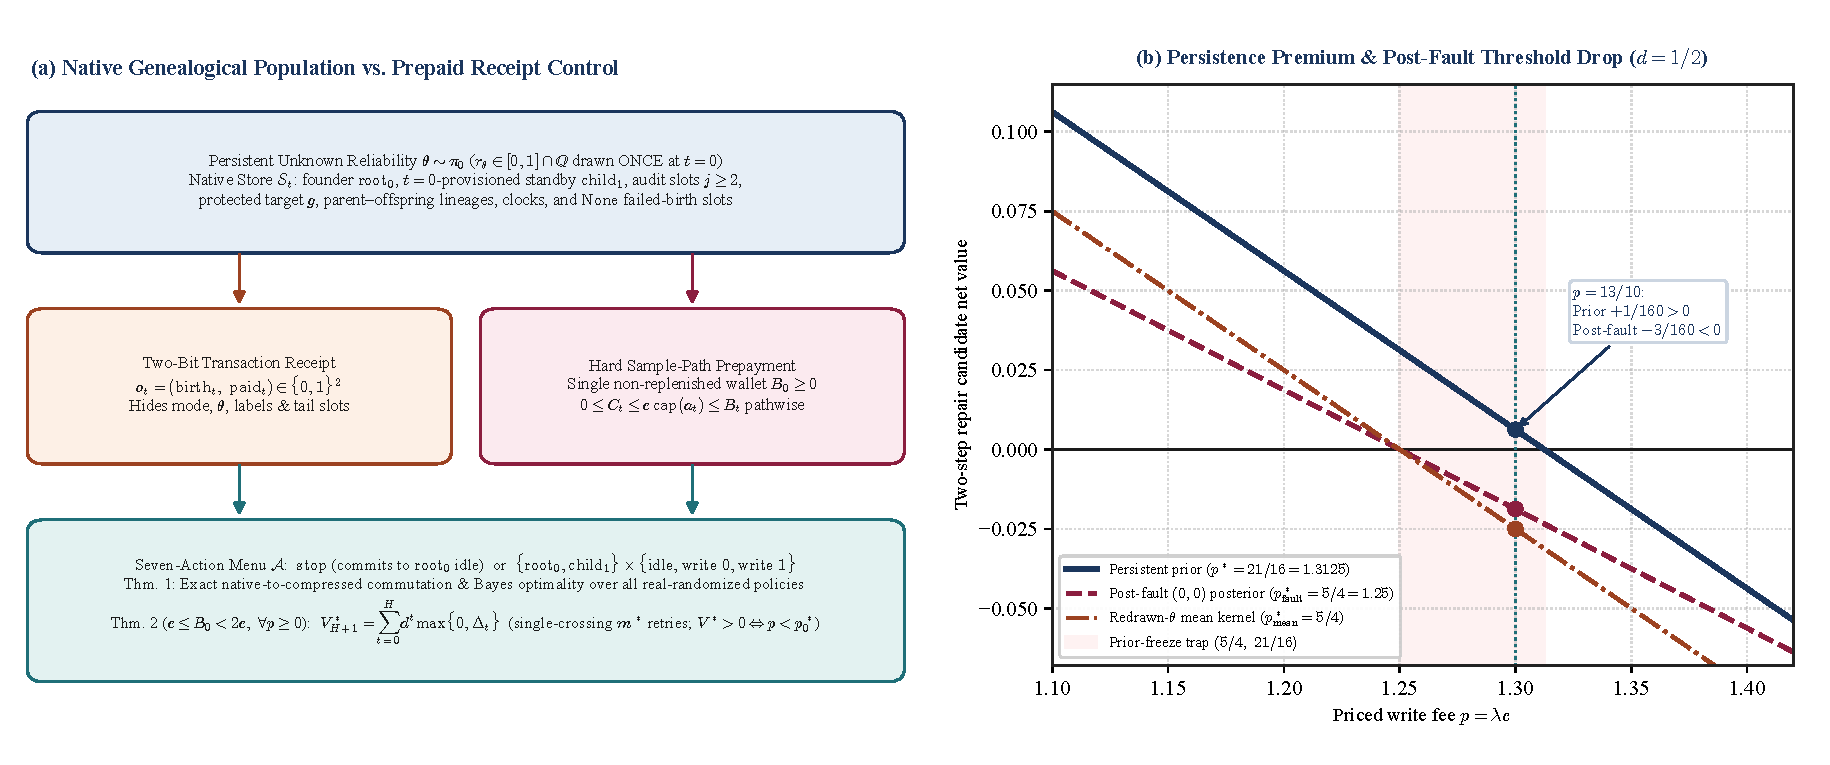
\includegraphics[width=0.99\linewidth,height=\textheight,keepaspectratio,alt={Native
genealogical population protocol and exact two-step repair-threshold
geometry. (a) Separation between the unbounded native genealogical store
\textbackslash mathcal\{S\}\_t and the controller's two-bit
post-transaction receipt interface o\_t = (\textbackslash
mathrm\{birth\}\_t, \textbackslash mathrm\{paid\}\_t) under hard
sample-path prepayment B\_t \textbackslash ge
c\textbackslash,\textbackslash mathrm\{cap\}(a\_t). (b) Exact two-step
repair candidate net value as a function of priced write fee p =
\textbackslash lambda c under equal prior weights on r\_\textbackslash
theta \textbackslash in \textbackslash\{1/4, 3/4\textbackslash\} and d =
1/2 (Theorems 2 and 3), showing the persistence variance premium
d\textbackslash,\textbackslash mathrm\{Var\}(r\_\textbackslash theta) =
1/32 over a step-redrawn mean kernel and the strict post-fault threshold
contraction from 21/16 to 5/4 creating the prior-freeze trap on (5/4,
21/16).}]{figures/fig1_architecture_and_thresholds.pdf}
\caption{Native genealogical population protocol and exact two-step
repair-threshold geometry. (a) Separation between the unbounded native
genealogical store \(\mathcal{S}_t\) and the controller's two-bit
post-transaction receipt interface
\(o_t = (\mathrm{birth}_t, \mathrm{paid}_t)\) under hard sample-path
prepayment \(B_t \ge c\,\mathrm{cap}(a_t)\). (b) Exact two-step repair
candidate net value as a function of priced write fee \(p = \lambda c\)
under equal prior weights on \(r_\theta \in \{1/4, 3/4\}\) and
\(d = 1/2\) (Theorems 2 and 3), showing the persistence variance premium
\(d\,\mathrm{Var}(r_\theta) = 1/32\) over a step-redrawn mean kernel and
the strict post-fault threshold contraction from \(21/16\) to \(5/4\)
creating the prior-freeze trap on \((5/4, 21/16)\).}
\end{figure}

\section{Persistence variance premium, post-fault posterior contraction,
and value of
information}\label{persistence-variance-premium-post-fault-posterior-contraction-and-value-of-information}

Writing \(\mu_k := \mathbb{E}_{\pi_0}[r_\theta^k]\) for the \(k\)-th
prior moment of the persistent reliability \(r_\theta\), Theorem 2
specializes at total horizons \(2\), \(3\), and \(4\) (\(B_0 = c\)) to
the explicit moment formulas \[\begin{aligned}
V_2^* &= \max\bigl\{0,\ \mu_1(1 - p) + d\,\mu_2\bigr\}, && p \ge 1, \\
V_3^* &= \max\bigl\{0,\ \mu_1(1 - p) + (d + d^2)\mu_2\bigr\}, && p \ge 1 + d, \\
V_4^* &= \max\bigl\{0,\ \mu_1(1 - p) + (d + d^2)\mu_2 + d^3(2\mu_3 - \mu_4)\bigr\}, && p \ge 1 + d + d^2.
\end{aligned}\] Comparing these exact expressions against restricted
information regimes---stepwise parameter redrawing, frozen priors after
a fault, open-loop continuation without receipt feedback, and omniscient
\(\theta\)-revelation---yields four sharp structural laws of Bayesian
adaptive maintenance
\citep{blackwell1953, howard1966, easleyKiefer1988, aghion1991, ross2011}.

\Needspace{24\baselineskip}

{\def\LTcaptype{none} % do not increment counter
\begin{longtable}[]{@{}
  >{\raggedright\arraybackslash}p{(\linewidth - 4\tabcolsep) * \real{0.3333}}
  >{\raggedright\arraybackslash}p{(\linewidth - 4\tabcolsep) * \real{0.3333}}
  >{\raggedright\arraybackslash}p{(\linewidth - 4\tabcolsep) * \real{0.3333}}@{}}
\toprule\noalign{}
\begin{minipage}[b]{\linewidth}\raggedright
Structural Contrast
\end{minipage} & \begin{minipage}[b]{\linewidth}\raggedright
Exact Formula / Threshold Identity
\end{minipage} & \begin{minipage}[b]{\linewidth}\raggedright
Concrete Verified Rational Witness (\(B_0 = c = 1\))
\end{minipage} \\
\midrule\noalign{}
\endhead
\bottomrule\noalign{}
\endlastfoot
Persistent vs.~redrawn \(\theta\) (\(H=2\)) &
\(V_{2,\mathrm{repair}} - V_{2,\mathrm{redraw}} = d(\mu_2 - \mu_1^2) = d\,\mathrm{Var}(r_\theta)\)
& \(r \in \{1/4, 3/4\}\) eq., \(d=1/2, p=13/10\): \(+1/160\)
vs.~\(-1/40\) \\
Post-fault \((0,0)\) threshold drop &
\(\Delta p^* = d\frac{\mu_1\mu_3 - \mu_2^2}{\mu_1(\mu_1 - \mu_2)} > 0\)
(\(0 < r_0 < r_1 < 1\)) & Threshold drops \(21/16 \to 5/4\); retry at
\(p=13/10\) gives \(-3/160\) \\
Prior-freeze loss (\(H=3, p < 1+d\)) &
\(V_3^* - J_3(\pi_{\mathrm{freeze}}) > 0\) for
\(p \in (p_{\mathrm{fault}}^*, p_{\mathrm{prior}}^*)\) &
\(r \in \{1/4, 3/4\}\) eq., \(d=1/2, p=13/10\):
\(27/320 - 51/640 = 3/640\) \\
Two-body vs.~root-only (\(H=3\)) &
\((d + d^2)\mu_2 - (d\mu_2 + d^2\mu_3) = d^2(\mu_2 - \mu_3)\) &
\(r \in \{1/4, 3/4\}\) eq., \(d=3/4, p=7/4\): \(+9/256\)
vs.~\(-9/512\) \\
Receipt feedback vs.~open-loop (\(H=4\)) & Raw continuation gap
\(d^3\mathbb{E}[r_\theta^3(1 - r_\theta)] \ge 0\) &
\(r \in \{3/4, 7/8\}\) eq., \(d=3/4, p=37/16\):
\(\Delta = 20925/524288\) \\
Post-repair \(\theta\)-revelation (\(\mathrm{EVPI}_{\mathrm{post}}\)) &
\(U_2(r_\theta, d, H)\) attained uniformly by \texttt{freeSchedule} &
\(\mathrm{EVPI}_{\mathrm{post}} = 0\) for \emph{every} prior \(\pi_0\)
and horizon \(H \ge 0\) \\
\end{longtable}
}

Table 1. Exact analytical decompositions and rational witnesses
separating parameter persistence, Bayesian fault updating, two-body
dispatch, receipt feedback, and post-repair parameter revelation.

\textbf{Theorem 3 (Persistence premium, post-fault threshold
contraction, feedback gain, and zero post-repair EVPI).} \emph{Under the
model of Theorem 1 with \(B_0 = c\):}

\begin{enumerate}
\def\labelenumi{\arabic{enumi}.}
\tightlist
\item
  \textbf{Persistence variance premium.} \emph{At total horizon \(2\),
  replacing persistent \(\theta \sim \pi_0\) by an i.i.d. redraw
  \(\theta_t \sim \pi_0\) at each step replaces
  \(\mu_2 = \mathbb{E}[r_\theta^2]\) by \(\mu_1^2\), reducing the
  initial-repair candidate value by
  \(d(\mu_2 - \mu_1^2) = d\,\mathrm{Var}(r_\theta) \ge 0\) (strictly
  positive whenever \(d > 0\) and \(\mathrm{Var}(r_\theta) > 0\)). Under
  equal prior weights on \(r \in \{1/4, 3/4\}\) with \(d = 1/2\) and
  \(p = 13/10\), persistent optimal value is \(V_2^* = 1/160 > 0\),
  whereas the redrawn mean-kernel repair value is \(-1/40 < 0\).}
\item
  \textbf{Strict post-fault repair-threshold contraction.} \emph{Suppose
  \(\mu_1 < 1\). Conditioning on an uncharged initial fault receipt
  \(o_0 = (0,0)\) after \((0, \mathrm{write}_g)\) leaves wallet
  \(B_1 = c\) unspent and updates the posterior moments to}
  \[\mu'_k := \mathbb{E}\bigl[r_\theta^k \mid o_0 = (0,0)\bigr] = \frac{\mu_k - \mu_{k+1}}{1 - \mu_1}, \qquad k \ge 1.\]
  \emph{For any nondegenerate two-point prior assigning weight
  \(w \in (0,1)\) to \(r_0\) and \(1 - w\) to \(r_1\) with
  \(0 < r_0 < r_1 < 1\),}
  \[\mu_1\mu_3 - \mu_2^2 = w(1 - w) r_0 r_1 (r_0 - r_1)^2 > 0.\]
  \emph{Consequently, for every \(d > 0\), the two-step repair
  positivity threshold strictly drops after a fault:}
  \[p_{\mathrm{fault}}^*(1) := 1 + d\,\frac{\mu'_2}{\mu'_1} = 1 + d\,\frac{\mu_2 - \mu_3}{\mu_1 - \mu_2} < 1 + d\,\frac{\mu_2}{\mu_1} = p_{\mathrm{prior}}^*(1).\]
  \emph{At \(w = 1/2\), \((r_0, r_1) = (1/4, 3/4)\), and \(d = 1/2\),
  the threshold drops from \(21/16\) to \(5/4\); at
  \(p = 13/10 \in (5/4, 21/16)\) and total horizon \(3\) (outside the
  high-price regime since \(13/10 < 1 + 1/2\)), the general dynamic
  program achieves \(V_3^* = 27/320\) by halting after \((0,0)\),
  whereas freezing the prior and retrying yields \(51/640\), incurring
  exact loss \(3/640\).}
\item
  \textbf{Open-loop sufficiency at \(H=3\) versus strict
  receipt-feedback gain at \(H=4\).} \emph{At total horizon \(3\)
  (\(B_0 = c\), \(p \ge 1 + d\)), the open-loop action sequence
  \([(0, \mathrm{write}_g), (0, \mathrm{idle}), (1, \mathrm{idle})]\)
  already achieves \(\mu_1(1-p) + (d + d^2)\mu_2 = V_3^*\) whenever
  positive (e.g., \(V_3^* = 9/256\) at
  \(r \in \{1/4, 3/4\}, d = 3/4, p = 7/4\), whereas restricting dispatch
  to \texttt{root0} alone yields \(-9/512 < 0\)). At total horizon
  \(4\), by contrast, after initial repair succeeds and exhausts the
  wallet, the maximum continuation value over all predetermined
  three-step open-loop sequences in
  \(\{(0, \mathrm{idle}), (1, \mathrm{idle})\}^3\) is
  \(r + dr + d^2 r^2\) (attained by alternating
  \((0, \mathrm{idle}), (1, \mathrm{idle}), (0, \mathrm{idle})\)),
  whereas receipt-adaptive switching achieves
  \(U_2(r, d, 3) = r + dr + d^2(2r^2 - r^3)\), yielding the nonnegative
  raw feedback advantage}
  \[\Delta_{\mathrm{raw}}^{(4)} := d^3\,\mathbb{E}_{\pi_0}\!\bigl[r_\theta^3(1 - r_\theta)\bigr] \ge 0,\]
  \emph{which is strictly positive iff \(d > 0\) and
  \(\mathbb{P}_{\pi_0}(0 < r_\theta < 1) > 0\). At equal weights on
  \(r \in \{3/4, 7/8\}\), \(d = 3/4\), and
  \(p = 37/16 \ge 1 + 3/4 + 9/16\), both candidates are strictly
  positive with \(V_4^* = 39525 / 524288\), open-loop optimum
  \(V_{4,\mathrm{open}}^* = 2325 / 65536\), and exact net feedback gain
  \(\Delta^{(4)} = 20925 / 524288\).}
\item
  \textbf{Exact zero post-repair value of \(\theta\)-revelation.}
  \emph{For every remaining horizon \(n \in \mathbb{N}\) after a
  successful repair leaves two intact units and exhausted wallet
  \(B = 0\), the parameter-blind receipt policy \texttt{freeSchedule}
  attains the \(\theta\)-omniscient continuation optimum
  \(U_2(r_\theta, d, n)\) pointwise for every \(r_\theta \in [0,1]\).
  Hence the expected value of perfect information on \(\theta\) in that
  continuation subgame is identically zero
  (\(\mathrm{EVPI}_{\mathrm{post}} = 0\)), and any positively priced
  auxiliary read of \(\theta\) strictly reduces expected net payoff.}
\end{enumerate}

Theorem 3 (proved in Appendix A.3) cleanly disentangles \emph{state
estimation} from \emph{parameter learning}
\citep{striebel1965, kumarVaraiya1986, krishnamurthy2016}. Why does
adaptive feedback create strictly positive value \(20925 / 524288\) at
\(H = 4\) even though learning \(\theta\) after repair has value \(0\)?
Because at step \(t = 1\) (idling \texttt{root0}) and step \(t = 2\)
(idling \texttt{child1}), an open-loop sequence cannot know \emph{which}
of the two bodies suffered a fault on step \(1\): if \texttt{root0}
faulted on step \(1\) while \texttt{child1} survived step \(2\)
(probability \((1 - r)r\)), returning blindly to \texttt{root0} on step
\(3\) wastes the final step on a damaged body, whereas reading the
step-\(1\) birth receipt routes step \(3\) to the surviving body
\texttt{child1}, gaining \(d^3 r^3(1 - r)\). Notice also that optimizing
net discounted payoff \(J_H\) is distinct from maximizing event
probabilities: in the \(H=2\) and \(H=3\) positive witnesses above,
\(\mathbb{P}(\sum_t \mathrm{birth}_t \ge 1) = 1/2\), and in the \(H=4\)
witness it is \(13/16\).

\section{Informative zero receipts, counting posteriors, and joint
all-action
sufficiency}\label{informative-zero-receipts-counting-posteriors-and-joint-all-action-sufficiency}

\subsection{Separating informative fault observations from deterministic
zero
receipts}\label{separating-informative-fault-observations-from-deterministic-zero-receipts}

When \(B_0 \ge 2c\) or \(p < S_H(d)\), multiple paid repairs and
mid-horizon retries become feasible, so closed-form single-write
formulas no longer apply and full dynamic programming is required. Over
the general belief space \(\Delta_{\mathbb{Q}}(\mathcal{W}(\Theta))\),
tracking finitely supported world beliefs across quaternary receipts and
seven actions generates a tree of size up to \(28^H\)
\citep{papadimitriouTsitsiklis1987, cassandra1997, hauskrecht2000}. To
compress this decision process \emph{without approximation loss}
\citep{liWalshLittman2006, subramanian2022}, we ask: what minimal
operational memory computed purely from public actions and two-bit
receipts \((a_t, o_t)\) suffices to reconstruct both the current
dispatchable physical configuration and the exact Bayesian posterior
over \(\Theta\) across \emph{all} real-randomized policies?

First, define the finite 24-element \emph{local observer state}
\(q = (x_0, x_1, \mathrm{stopped}, \mathrm{fresh}) \in Q := \{0,1\} \times \{\mathrm{None}, 0, 1\} \times \{0,1\} \times \{0,1\}\)
(\(|Q| = 2 \times 3 \times 2 \times 2 = 24\)), initialized at
\(q_{\mathrm{init}}(g) := (\neg g, \mathrm{None}, 0, 1)\). Here
\(x_0 \in \{0,1\}\) tracks the physical bit of \texttt{root0},
\(x_1 \in \{\mathrm{None}, 0, 1\}\) tracks whether slot \texttt{child1}
is permanently \texttt{None} or holds a unit with bit \(0\) or \(1\),
\(\mathrm{stopped} \in \{0,1\}\) tracks the permanent stop latch, and
\(\mathrm{fresh} \in \{0,1\}\) holds only at \(t = 0\) prior to the
first append (since only the \(t=0\) transaction allocates slot \(1\);
if \(o_0 = (0, \cdot)\), slot \(1\) becomes \texttt{None} forever). From
\((g, q, a, o)\) alone---without inspecting the hidden world---the
observer updates \(q' = \mathrm{upd}(g, q, a, o)\) deterministically:
writing
\((j_{\mathrm{eff}}, \alpha_{\mathrm{eff}}) = \mathrm{eff}(q.\mathrm{stopped}, a)\)
and \(\beta(g, \mathrm{birth}) := g\) if \(\mathrm{birth} = 1\) else
\(\neg g\), \[\begin{aligned}
x'_0 &:= \begin{cases} x_0, & j_{\mathrm{eff}} = 1, \\ \beta(g, o_1), & j_{\mathrm{eff}} = 0, \end{cases}
&
x'_1 &:= \begin{cases} g, & q.\mathrm{fresh} = 1 \land o_1 = 1, \\ \mathrm{None}, & q.\mathrm{fresh} = 1 \land o_1 = 0, \\ \mathrm{Option.map}(\lambda\_.\,\beta(g, o_1), x_1), & q.\mathrm{fresh} = 0 \land j_{\mathrm{eff}} = 1, \\ x_1, & q.\mathrm{fresh} = 0 \land j_{\mathrm{eff}} = 0, \end{cases}
\end{aligned}\] with
\(\mathrm{stopped}' := q.\mathrm{stopped} \lor \mathbf{1}_{\{a = \mathrm{stop}\}}\)
and \(\mathrm{fresh}' := 0\).

Second, given \((g, q, a)\), let
\(o_{\mathrm{norm}}(g, q, a) \in \{0,1\}^2\) denote the deterministic
receipt that would occur under normal mode \(m = 1\): if the selected
slot in \(q\) is \texttt{None}, \(o_{\mathrm{norm}} = (0,0)\); if the
selected slot holds bit \(x\),
\(o_{\mathrm{norm}} = (\mathbf{1}_{\{x_{\mathrm{cand}}(x, \alpha_{\mathrm{eff}}) = g\}},\, \mathbf{1}_{\{\alpha_{\mathrm{eff}} \neq \mathrm{idle}\}})\).
Under fault mode \(m = 0\), the receipt is \emph{always} \((0,0)\).
Summing out the fair hidden label \(\ell \in \{0,1\}\) gives the exact
single-step marginal receipt likelihood at reliability \(r \in [0,1]\):
\[L_r(o \mid g, q, a) := r\,\mathbf{1}_{\{o = o_{\mathrm{norm}}(g, q, a)\}} + (1 - r)\,\mathbf{1}_{\{o = (0,0)\}}.\]
Observe the critical dichotomy revealed by Table 2: whenever
\(o_{\mathrm{norm}}(g, q, a) = (0,0)\)---which occurs precisely when
idling a damaged slot (\(x = \neg g\)) or dispatching an absent
\texttt{child1} (\(x_1 = \mathrm{None}\))---\emph{both} normal and fault
modes emit \((0,0)\), so \(L_r((0,0) \mid g, q, a) = r + (1 - r) = 1\)
for \emph{every} \(r \in [0,1]\).

\Needspace{24\baselineskip}

{\def\LTcaptype{none} % do not increment counter
\begin{longtable}[]{@{}
  >{\raggedright\arraybackslash}p{(\linewidth - 8\tabcolsep) * \real{0.1818}}
  >{\raggedright\arraybackslash}p{(\linewidth - 8\tabcolsep) * \real{0.1818}}
  >{\centering\arraybackslash}p{(\linewidth - 8\tabcolsep) * \real{0.2273}}
  >{\centering\arraybackslash}p{(\linewidth - 8\tabcolsep) * \real{0.2273}}
  >{\raggedright\arraybackslash}p{(\linewidth - 8\tabcolsep) * \real{0.1818}}@{}}
\toprule\noalign{}
\begin{minipage}[b]{\linewidth}\raggedright
Selected Slot State in \(q\)
\end{minipage} & \begin{minipage}[b]{\linewidth}\raggedright
Effective Action \(\alpha_{\mathrm{eff}}\)
\end{minipage} & \begin{minipage}[b]{\linewidth}\centering
Normal Receipt \(o_{\mathrm{norm}}\)
\end{minipage} & \begin{minipage}[b]{\linewidth}\centering
Fault Receipt
\end{minipage} & \begin{minipage}[b]{\linewidth}\raggedright
Informative? (\(\Delta s + \Delta f = 1\))
\end{minipage} \\
\midrule\noalign{}
\endhead
\bottomrule\noalign{}
\endlastfoot
Existing slot (\(x \in \{0,1\}\)) & \(\mathrm{write}_g\) & \((1, 1)\) &
\((0, 0)\) & \textbf{Yes}: \((1,1) \Rightarrow \Delta s=1\);
\((0,0) \Rightarrow \Delta f=1\) \\
Existing slot (\(x \in \{0,1\}\)) & \(\mathrm{write}_{\neg g}\) &
\((0, 1)\) & \((0, 0)\) & \textbf{Yes}: \((0,1)\) (charged)
\(\Rightarrow \Delta s=1\); \((0,0) \Rightarrow \Delta f=1\) \\
Healthy slot (\(x = g\)) & \(\mathrm{idle}\) & \((1, 0)\) & \((0, 0)\) &
\textbf{Yes}: \((1,0) \Rightarrow \Delta s=1\);
\((0,0) \Rightarrow \Delta f=1\) \\
Damaged slot (\(x = \neg g\)) & \(\mathrm{idle}\) & \((0, 0)\) &
\((0, 0)\) & \textbf{No}: \(L_r((0,0)) \equiv 1\)
(\(\Delta s = \Delta f = 0\)) \\
Absent slot (\(x_1 = \mathrm{None}\)) & Any \(\alpha_{\mathrm{eff}}\) &
\((0, 0)\) & \((0, 0)\) & \textbf{No}: \(L_r((0,0)) \equiv 1\)
(\(\Delta s = \Delta f = 0\)) \\
\end{longtable}
}

Table 2. Exact five-case classification of normal versus fault receipts
(\texttt{RegisterDecisionObserver}), showing why damaged-slot idles and
absent-slot requests produce uninformative zero receipts that must not
increment the fault counter \(f\).

Define the Boolean predicate
\(\mathrm{informative}(g, q, a) :\iff o_{\mathrm{norm}}(g, q, a) \neq (0,0)\)
(equivalently, \(o_{\mathrm{norm},1} \lor o_{\mathrm{norm},2} = 1\)),
and define the step increments
\[\Delta s(g, q, a, o) := \mathbf{1}_{\{\mathrm{informative}(g,q,a) \land o \neq (0,0)\}}, \qquad
\Delta f(g, q, a, o) := \mathbf{1}_{\{\mathrm{informative}(g,q,a) \land o = (0,0)\}}.\]
Calling \(o\) \emph{compatible} with \((g, q, a)\) if
\(o \in \{o_{\mathrm{norm}}(g, q, a),\, (0,0)\}\), the marginal
likelihood factors identically for \emph{all} \(r \in [0,1]\) (retaining
the convention \(0^0 := 1\) at endpoint rates \(r \in \{0,1\}\)) as
\[L_r(o \mid g, q, a) = \mathbf{1}_{\{\mathrm{compatible}(g, q, a, o)\}}\, r^{\Delta s(g, q, a, o)} (1 - r)^{\Delta f(g, q, a, o)}.\]
Folding \((a_t, o_t)\) chronologically along any history
\(h \in (\mathcal{A} \times \mathcal{O})^*\) from
\((0, 0, 0, 0, q_{\mathrm{init}}(g))\) produces the five-coordinate
operational summary
\[\sigma(h) := \bigl(t(h),\ q(h),\ s(h),\ f(h),\ k(h)\bigr) \in \mathbb{N} \times Q \times \mathbb{N} \times \mathbb{N} \times \mathbb{N},\]
where \(t(h) = |h|\) is elapsed time, \(s(h)\) and \(f(h)\) are
cumulative informative normal and fault counts, and
\(k(h) := \sum_{u < |h|} \mathbf{1}_{\{o_{u,2} = 1\}}\) is cumulative
paid writes. Setting
\(w_\theta(s, f) := \pi_0(\theta)\, r_\theta^s (1 - r_\theta)^f\) and
\(Z(s, f) := \sum_{\theta \in \Theta} w_\theta(s, f)\), we obtain
universal posterior sufficiency across \emph{all} real-randomized
policies \citep{halmosSavage1949, dynkin1978}.

\textbf{Theorem 4 (Universal counting-posterior factorization under
arbitrary real-randomized policies).} \emph{Let \(\pi\) be any causal
real-randomized full-history strategy (not assumed to factor through
\(\sigma\), and with arbitrary initial private memory independent of
\(\theta\) and \(\mathcal{S}_0\)). For every history
\(h = [(a_0, o_0), \dots, (a_{t-1}, o_{t-1})] \in (\mathcal{A} \times \mathcal{O})^t\):}

\begin{enumerate}
\def\labelenumi{\arabic{enumi}.}
\tightlist
\item
  \textbf{Likelihood factorization.} \emph{There exists a
  \(\theta\)-independent action-randomization factor
  \(\alpha_\pi(h) \in \mathbb{R}_{\ge 0}\) (the product of \(\pi\)'s
  conditional action probabilities along \(h\)) such that for every
  \(\theta \in \Theta\), the exact native joint probability of
  \((\theta, h)\) is}
  \[\mathbb{P}_{\pi_0, \pi}(\theta, h) = \alpha_\pi(h)\,\mathbf{1}_{\{\mathrm{compat}(h)\}}\, \pi_0(\theta)\, r_\theta^{s(h)} (1 - r_\theta)^{f(h)},\]
  \emph{where \(\mathrm{compat}(h)\) holds iff every step \((a_u, o_u)\)
  in \(h\) is compatible with \((g, q_u, a_u)\). This holds
  unconditionally for all \(\pi_0(\theta) \ge 0\) and all endpoint rates
  \(r_\theta \in [0,1]\) (with \(0^0 = 1\)).}
\item
  \textbf{Exact cancellation on positive-mass histories.} \emph{Whenever
  \(\mathbb{P}_{\pi_0, \pi}(h) = \sum_\theta \mathbb{P}_{\pi_0, \pi}(\theta, h) > 0\),
  necessarily \(\mathrm{compat}(h)\) holds, \(\alpha_\pi(h) > 0\), and
  \(Z(s(h), f(h)) > 0\), so \(\alpha_\pi(h)\) cancels identically and
  the exact conditional posterior is}
  \[\mathbb{P}_{\pi_0, \pi}(\theta \mid h) = \frac{\pi_0(\theta)\, r_\theta^{s(h)} (1 - r_\theta)^{f(h)}}{Z\bigl(s(h), f(h)\bigr)} \in \mathbb{Q} \qquad (\forall \theta \in \Theta).\]
\end{enumerate}

\subsection{Joint all-action sufficiency and necessary versus removable
history
distinctions}\label{joint-all-action-sufficiency-and-necessary-versus-removable-history-distinctions}

Combining local-observer reconstruction with Theorem 4 shows that
\(\sigma = (t, q, s, f, k)\) is a \emph{jointly sufficient decision
state} across the entire action menu
\citep{striebel1965, burkeRosenblatt1958, kemenySnell1960, givanDeanGreig2003},
while reachable three-step trajectories prove that neither \((s,f)\) nor
\(q\) can be dropped and that sufficiency is strictly indexed to the
permitted action menu (Figure 2).

\textbf{Theorem 5 (Joint all-action sufficiency of
\(\sigma = (t, q, s, f, k)\) and three-way sharpness separations).}
\emph{Under the hypotheses of Theorem 1:}

\begin{enumerate}
\def\labelenumi{\arabic{enumi}.}
\tightlist
\item
  \textbf{Joint single-step and multi-step Bellman sufficiency.}
  \emph{If two positive-mass permitted histories \(h_1, h_2\) at
  remaining horizon \(n = H - t\) satisfy
  \(\sigma(h_1) = \sigma(h_2) = (t, q, s, f, k)\), then their literal
  remaining balances coincide (\(B(h_1) = B(h_2) = B_0 - kc \ge 0\)),
  their feasible menus \(\mathrm{menu}(c, B)\) coincide, and for every
  action \(a \in \mathrm{menu}(c, B)\), their one-step joint
  distributions over
  \((o_t,\, \sigma(h_i \mathbin{+\!+} [(a, o_t)]),\, \mathrm{birth}_t,\, C_t,\, B_{t+1})\)
  are identical. By backward induction (\texttt{StepRefinement}), the
  summary dynamic program over \((n, \sigma)\) has the exact same
  optimal value \(V_H^*(b_0, B_0)\) as the full world-belief dynamic
  program over all supported-admissible real-randomized full-history
  policies.}
\item
  \textbf{Insufficiency of the physical Markov state \((t, q, B)\).}
  \emph{Under equal prior weights on \(r \in \{1/4, 3/4\}\) and
  \(B_0 = c = 1\), execute the fixed three-step sequence
  \([(0, \mathrm{write}_g), (0, \mathrm{idle}), (0, \mathrm{idle})]\).
  Reachable histories} \[\begin{aligned}
  h_A &:= \bigl[((0,\mathrm{write}_g),(1,1)),\ ((0,\mathrm{idle}),(1,0)),\ ((0,\mathrm{idle}),(0,0))\bigr], \\
  h_B &:= \bigl[((0,\mathrm{write}_g),(1,1)),\ ((0,\mathrm{idle}),(0,0)),\ ((0,\mathrm{idle}),(0,0))\bigr]
  \end{aligned}\] \emph{have strictly positive prior probabilities
  \(3/32\) and \(3/16\), and reach the identical elapsed time \(t = 3\),
  exhausted wallet \(B_3 = 0\), and local body state
  \(q_* = (\neg g, \mathrm{Some}(g), 0, 0)\). Yet because \(h_B\)'s
  third step idles an already-damaged \texttt{root0} (\(\Delta f = 0\)),
  \(\sigma(h_A)\) has \((s,f) = (2,1)\) (\(\pi_{h_A}(1/4) = 1/4\))
  whereas \(\sigma(h_B)\) has \((s,f) = (1,1)\)
  (\(\pi_{h_B}(1/4) = 1/2\)), yielding strictly distinct next-step birth
  probabilities under \((1, \mathrm{idle})\):
  \(\mathbb{P}(\mathrm{birth}_3 = 1 \mid h_A) = 5/8 \neq 1/2 = \mathbb{P}(\mathrm{birth}_3 = 1 \mid h_B)\).}
\item
  \textbf{Genuine genealogy-erasing history merger and menu-relative
  boundary.} \emph{Under the same prior and wallet, reachable three-step
  histories} \[\begin{aligned}
  m_A &:= \bigl[((0,\mathrm{write}_g),(1,1)),\ ((0,\mathrm{idle}),(0,0)),\ ((1,\mathrm{idle}),(1,0))\bigr], \\
  m_B &:= \bigl[((0,\mathrm{write}_g),(1,1)),\ ((1,\mathrm{idle}),(1,0)),\ ((0,\mathrm{idle}),(0,0))\bigr]
  \end{aligned}\] \emph{(each with probability \(3/32\) and posterior
  \(\pi(1/4) = 1/4\)) share the exact complete summary
  \(\sigma(m_A) = \sigma(m_B) = (3, q_*, 2, 1, 1)\) and induce identical
  future joint laws across all seven actions in \(\mathcal{A}\), even
  though their native population stores have distinct slot layouts}
  \[[\mathrm{Some}(\neg g),\, \mathrm{Some}(g),\, \mathrm{None},\, \mathrm{Some}(g)]
  \;\neq\;
  [\mathrm{Some}(\neg g),\, \mathrm{Some}(g),\, \mathrm{Some}(g),\, \mathrm{None}],\]
  \emph{distinct parent--offspring identity records, and distinct
  realized past discounted payoffs (\(1 - p + d^2\) vs.~\(1 - p + d\)).
  However, if the action menu is enlarged with \texttt{(2,\ idle)}
  (dispatching slot \(2\)), future birth probabilities diverge
  immediately to \(0\) after \(m_A\) versus \(r_\theta\) (mean \(5/8\))
  after \(m_B\).}
\end{enumerate}

\begin{figure}
\centering
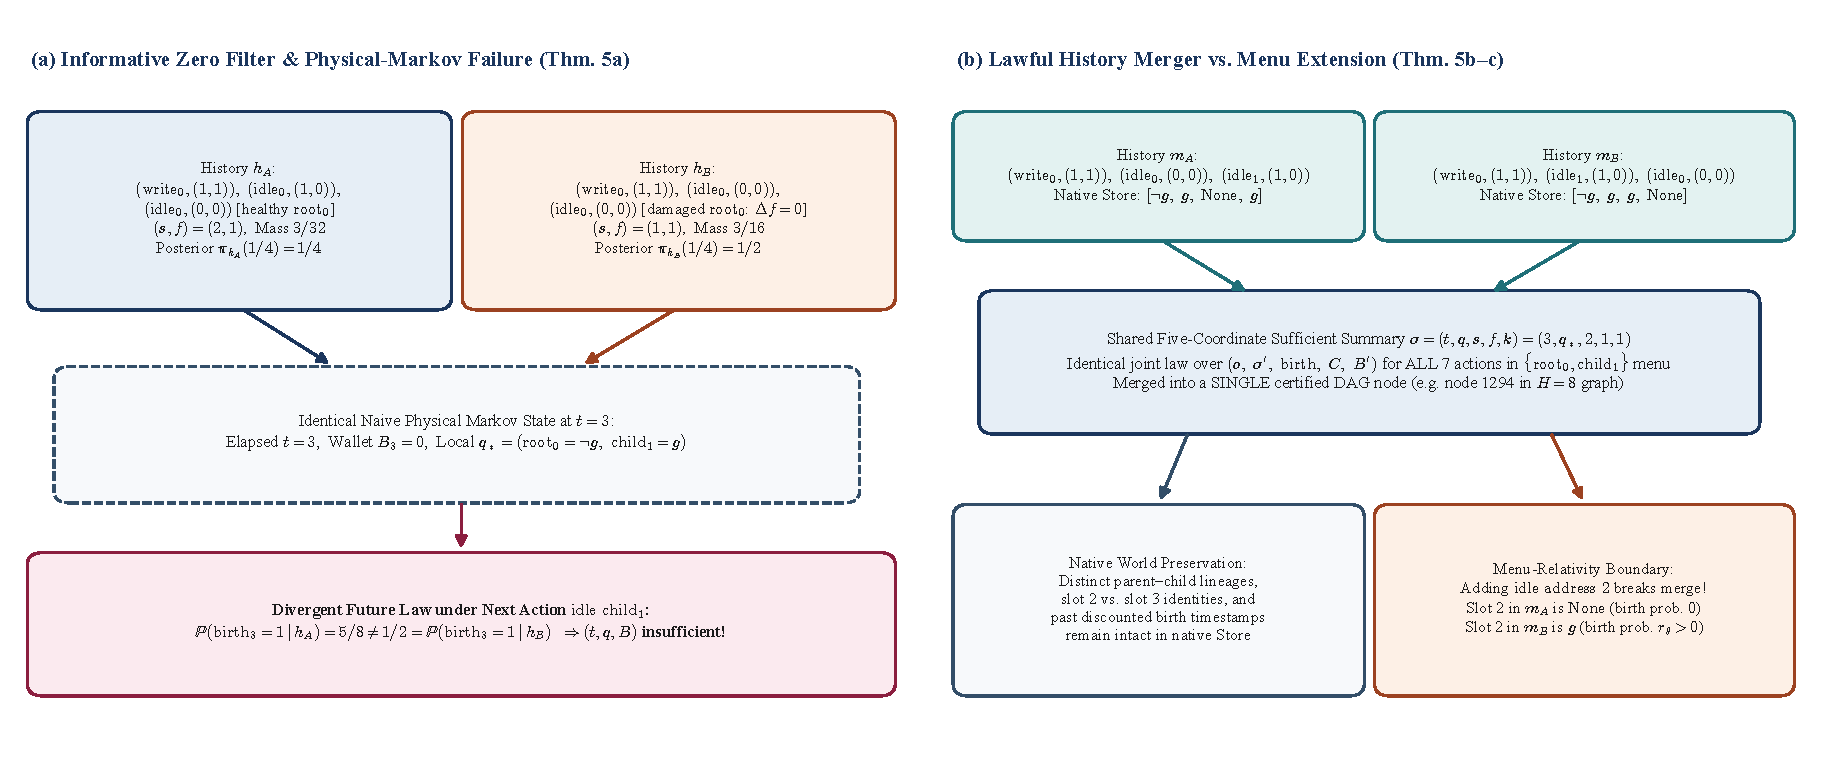
\includegraphics[width=0.99\linewidth,height=\textheight,keepaspectratio,alt={Informative
zero-receipt filtering, physical-Markov failure, and lawful
genealogy-erasing history merger (Theorems 4 and 5). (a) Reachable
histories h\_A and h\_B reach identical elapsed time t=3, wallet B\_3=0,
and local body state q\_* = (\textbackslash neg g, g) yet induce
distinct posteriors and next-step birth probabilities (5/8 vs.~1/2)
because h\_B's third-step zero receipt on a damaged root is
uninformative (\textbackslash Delta f = 0). (b) Reachable histories m\_A
and m\_B with non-isomorphic native genealogical tail stores share exact
five-coordinate summary \textbackslash sigma = (3, q\_*, 2, 1, 1) and
merge into a single certified decision-diagram node under the \{root0,
child1\} menu, while separating (0 vs.~r\_\textbackslash theta) if
slot-2 dispatch is
added.}]{figures/fig2_informative_counts_and_sufficiency.pdf}
\caption{Informative zero-receipt filtering, physical-Markov failure,
and lawful genealogy-erasing history merger (Theorems 4 and 5). (a)
Reachable histories \(h_A\) and \(h_B\) reach identical elapsed time
\(t=3\), wallet \(B_3=0\), and local body state \(q_* = (\neg g, g)\)
yet induce distinct posteriors and next-step birth probabilities
(\(5/8\) vs.~\(1/2\)) because \(h_B\)'s third-step zero receipt on a
damaged root is uninformative (\(\Delta f = 0\)). (b) Reachable
histories \(m_A\) and \(m_B\) with non-isomorphic native genealogical
tail stores share exact five-coordinate summary
\(\sigma = (3, q_*, 2, 1, 1)\) and merge into a single certified
decision-diagram node under the \protect\texttt{\{root0,\ child1\}}
menu, while separating (\(0\) vs.~\(r_\theta\)) if slot-2 dispatch is
added.}
\end{figure}

\section{All-action certifying decision diagrams and explicit polynomial
node
bounds}\label{all-action-certifying-decision-diagrams-and-explicit-polynomial-node-bounds}

\subsection{Separating untrusted memoized graph synthesis from
all-action certificate
checking}\label{separating-untrusted-memoized-graph-synthesis-from-all-action-certificate-checking}

Having shown in Theorem 5 that the five-coordinate summary
\(\sigma = (t, q, s, f, k)\) preserves exact joint single-step
transitions and full-history Bellman values across all legal actions,
how should an implementation construct, store, and \emph{verify} the
resulting shared policy graph? Standard decision-diagram planners in
stochastic control---such as algebraic decision diagrams in factored
MDPs \citep{bryant1986, bahar1997, hoey1999, boutilier2000},
finite-state controller search
\citep{littman1995, hansen1998, meuleau1999, poupartBoutilier2003},
point-based or Monte Carlo POMDP approximations
\citep{pineau2003, spaanVlassis2005, silverVeness2010}, and optimization
decision diagrams \citep{bergman2016}---typically interleave hash-table
memoization, pruning heuristics, and floating-point value updates inside
a single monolithic solver. Proving total correctness of mutable or
hash-indexed graph-building code directly inside a proof assistant can
be brittle and obscures the mathematical structure of the certificate.

Following the \emph{certifying algorithm} paradigm
\citep{blumKannan1995, mcconnell2011}, we decouple graph construction
into two strictly separated Lean modules---an untrusted generator
(\texttt{FiniteJointDecisionDAGGenerator}) and a trusted verifier
(\texttt{FiniteJointDecisionDAG}):

\begin{enumerate}
\def\labelenumi{\arabic{enumi}.}
\tightlist
\item
  \textbf{Untrusted memoized DAG generator (\texttt{generate}).} Given a
  problem instance specified by \((\Theta, \pi_0, r_\cdot, g)\) and
  \((c, B_0, \lambda, d, H)\), \texttt{generate} initializes an empty
  hash map keyed by \((n, \sigma)\)---where \(n = H - t\) is remaining
  horizon---and recursively expands positive-mass receipt successors
  \(m_\sigma^a(o) > 0\) for \emph{every} legal action
  \(a \in \mathrm{menu}(c, \max\{0, B_0 - kc\})\). Completed child nodes
  are appended bottom-up to a flat array
  \(G = [\mathrm{node}_0, \dots, \mathrm{node}_{N_H - 1}]\), so every
  parent edge stores only a bounded integer cursor
  \texttt{idx\ \textless{}\ G.size}. Whenever two distinct histories
  reach the same key \((n, \sigma)\), they reuse the identical array
  index without re-solving the subproblem or materializing the \(28^H\)
  tree.
\item
  \textbf{Trusted executable all-action certificate checker
  (\texttt{certify\ :\ Option\ Certified}).} Rather than trusting
  \texttt{generate}, the Boolean verifier \texttt{check} inspects the
  candidate array \(G\) and designated root index \texttt{root\_id}
  directly:

  \begin{itemize}
  \tightlist
  \item
    \emph{Key uniqueness and horizon binding:} Every stored row in \(G\)
    has a distinct key \((n_i, \sigma_i)\), and the root row matches
    \((H, \sigma_{\mathrm{init}})\) where
    \(\sigma_{\mathrm{init}} = (0, q_{\mathrm{init}}(g), 0, 0, 0)\).
  \item
    \emph{Terminal base check:} Every row with \(n_i = 0\) stores exact
    rational value \(v_i = 0\).
  \item
    \emph{Exhaustive all-action and positive-receipt check
    (\texttt{NodeValid}):} At every non-terminal row \((n_i, \sigma_i)\)
    with \(n_i > 0\), \texttt{check} enumerates \emph{all} legal actions
    \(a \in \mathrm{menu}(c, B(\sigma_i))\)---not merely the selected
    action \(a_i^*\)---verifies that \emph{every} receipt
    \(o \in \mathcal{O}\) with strictly positive counting-posterior mass
    \(m_{\sigma_i}^a(o) > 0\) appears in the row's edge table pointing
    to a valid index \(j < G.\mathrm{size}\) whose key equals
    \((n_i - 1, \mathrm{updStat}(g, \sigma_i, a, o))\), recomputes the
    exact rational \(Q\)-value
    \[Q_G(i, a) := \sum_{o : m_{\sigma_i}^a(o) > 0} m_{\sigma_i}^a(o)\Bigl[\bigl(\mathbf{1}_{\{o_1 = 1\}} - \lambda c \mathbf{1}_{\{o_2 = 1\}}\bigr) + d\, v_{\mathrm{target}(i, a, o)}\Bigr] \in \mathbb{Q},\]
    and verifies that
    \(v_i = \max_{a \in \mathrm{menu}(c, B(\sigma_i))} Q_G(i, a)\) and
    that \(a_i^*\) matches the first-occurring maximizer in the
    canonical order of \(\mathcal{A}\).
  \item
    \emph{Explicit domain bound check (\texttt{boundCheck}):} Every
    stored row in \(G\) satisfies \(n_i + t_i = H\),
    \(s_i + f_i \le t_i\), and \(k_i \le t_i\).
  \end{itemize}
\end{enumerate}

Only if all checks evaluate to \texttt{true} does \texttt{returned}
output \texttt{some\ res}; otherwise it returns \texttt{none}. Why must
\texttt{NodeValid} retain and check alternative suboptimal actions
inside \(G\)? Because a policy graph that stores \emph{only} the chosen
action \(a_i^*\) at each reachable node can verify what payoff \(a_i^*\)
achieves (\(J_H(G) = v_{\mathrm{root}}\)), \emph{but cannot certify that
no other legal action beats \(a_i^*\)}. Indeed, in our formalized
negative test (\texttt{OMITTED\_ALTERNATIVE\_REJECTION}), deleting a
single positive-probability successor edge of an unselected
\texttt{stop} action causes \texttt{certify} to reject the candidate
graph immediately.

\subsection{Quartic node ceiling, native cursor execution, and
multi-horizon rational
benchmarks}\label{quartic-node-ceiling-native-cursor-execution-and-multi-horizon-rational-benchmarks}

Once \texttt{certify} accepts \((G, \mathrm{root\_id})\), runtime
execution (\texttt{packedRun} / \texttt{nativeRun}) never unfolds
\texttt{G} back into a tree: at each tick \(t\), the controller
maintains only an integer node cursor \(i_t \in \{0, \dots, N_H - 1\}\),
issues the stored action \(a_{i_t}^* \in \mathcal{A}\) to the native
genealogical store \(\mathcal{S}_t\), receives
\(o_t = (\mathrm{birth}_t, \mathrm{paid}_t)\), advances \(i_{t+1}\)
along the certified edge for \((a_{i_t}^*, o_t)\), and falls back to an
explicit safe zero-fee action (\texttt{stop}) on any impossible
zero-mass branch (Figure 3).

\textbf{Theorem 6 (Soundness of certified shared decision diagrams,
pathwise native prepayment, and quartic size bound).} \emph{Suppose
\texttt{RegisterDecisionRepresentation.returned} outputs
\texttt{some\ res} with certified shared array \(G\), root index
\(i_{\mathrm{root}}\), and rational root value
\(v_{\mathrm{root}} \in \mathbb{Q}\) for horizon \(H \in \mathbb{N}\).}

\begin{enumerate}
\def\labelenumi{\arabic{enumi}.}
\tightlist
\item
  \textbf{Exact native attainment and full-history real-randomized
  optimality.} \emph{Executing \(G\) from \(i_{\mathrm{root}}\) directly
  against the native genealogical store \(\mathcal{S}_0\) produces exact
  expected discounted net payoff
  \(J_H^{\mathrm{native}}(G) = v_{\mathrm{root}} = V_H^*(b_0, B_0)\),
  dominating every supported-admissible real-randomized full-history
  strategy \(\pi\):
  \(J_H^{\mathrm{native}}(\pi) \le v_{\mathrm{root}}\). Along every run
  of length \(H\), native execution preserves \(L_H = 1 + H\) total
  slots (including \texttt{None} slots and post-\texttt{stop} ticks)
  alongside complete lineage and clock records.}
\item
  \textbf{Unconditional sample-path prepayment safety.} \emph{Even
  without invoking optimality of \(G\), menu-feasibility of every stored
  node action guarantees that on every positive-prior \(\theta\) and
  positive-weight primitive noise tape \((z_0, \dots, z_{H-1})\), every
  prefix \(m \le H\) satisfies pre-execution affordability
  \(c\,\mathrm{cap}(a_t) \le B_t\) (\(t < m\)) and literal balance
  conservation}
  \[B_m = B_0 - \sum_{t=0}^{m-1} C_t \ge 0, \qquad 0 \le \sum_{t=0}^{m-1} C_t \le B_0.\]
\item
  \textbf{Explicit quartic node-count ceiling.} \emph{Every accepted
  shared array \(G\)---counting all stored rows, including terminal rows
  and alternative-action upper-bound subgraphs---satisfies}
  \[N_H := G.\mathrm{size} \le 24\,(H + 1)^4.\]
\end{enumerate}

Theorem 6 (proved in Appendix A.6) replaces exponential
\((|\mathcal{A}||\mathcal{O}|)^H = 28^H\) history-table growth with a
machine-checked \(O(H^4)\) node guarantee. Notice why the exponent is
\(4\) rather than \(5\) even though \((n, \sigma) = (n, t, q, s, f, k)\)
has five integer coordinates plus \(q \in Q\): every reachable row
satisfies the horizon invariant \(n + t = H\), so the map
\((n, t, q, s, f, k) \mapsto (t, s, f, k, q) \in \{0, \dots, H\}^4 \times Q\)
is injective on \(G\), bounding
\(|G| \le |\{0, \dots, H\}|^4 \cdot |Q| = 24(H+1)^4\).

\Needspace{24\baselineskip}

{\def\LTcaptype{none} % do not increment counter
\begin{longtable}[]{@{}
  >{\raggedright\arraybackslash}p{(\linewidth - 10\tabcolsep) * \real{0.1600}}
  >{\raggedright\arraybackslash}p{(\linewidth - 10\tabcolsep) * \real{0.1600}}
  >{\centering\arraybackslash}p{(\linewidth - 10\tabcolsep) * \real{0.2000}}
  >{\raggedleft\arraybackslash}p{(\linewidth - 10\tabcolsep) * \real{0.1600}}
  >{\raggedleft\arraybackslash}p{(\linewidth - 10\tabcolsep) * \real{0.1600}}
  >{\raggedleft\arraybackslash}p{(\linewidth - 10\tabcolsep) * \real{0.1600}}@{}}
\toprule\noalign{}
\begin{minipage}[b]{\linewidth}\raggedright
Benchmark Instance (\(c = 1, g = 1\))
\end{minipage} & \begin{minipage}[b]{\linewidth}\raggedright
\((H, B_0, d, \lambda)\) \& Prior \(r_\theta\)
\end{minipage} & \begin{minipage}[b]{\linewidth}\centering
Exact Optimal Value \(V_H^*\)
\end{minipage} & \begin{minipage}[b]{\linewidth}\raggedleft
Cert. Nodes / Edges
\end{minipage} & \begin{minipage}[b]{\linewidth}\raggedleft
Exec. Nodes / Edges
\end{minipage} & \begin{minipage}[b]{\linewidth}\raggedleft
Raw Tree \(28^H\) vs.~\(24(H+1)^4\)
\end{minipage} \\
\midrule\noalign{}
\endhead
\bottomrule\noalign{}
\endlastfoot
1. Persistent two-step & \((2, 1, \frac{1}{2}, \frac{13}{10})\),
\(\{\frac{1}{4}, \frac{3}{4}\}\) eq. & \(\dfrac{1}{160}\) &
\(21\ /\ 43\) & \(6\ /\ 5\) & \(784\) vs.~\(1,944\) \\
2. Three-step backup & \((3, 1, \frac{3}{4}, \frac{7}{4})\),
\(\{\frac{1}{4}, \frac{3}{4}\}\) eq. & \(\dfrac{9}{256}\) &
\(52\ /\ 127\) & \(11\ /\ 10\) & \(21,952\) vs.~\(6,144\) \\
3. Three-step posterior & \((3, 1, \frac{1}{2}, \frac{13}{10})\),
\(\{\frac{1}{4}, \frac{3}{4}\}\) eq. & \(\dfrac{27}{320}\) &
\(52\ /\ 127\) & \(11\ /\ 10\) & \(21,952\) vs.~\(6,144\) \\
4. Four-step feedback & \((4, 1, \frac{3}{4}, \frac{37}{16})\),
\(\{\frac{3}{4}, \frac{7}{8}\}\) eq. & \(\dfrac{39525}{524288}\) &
\(104\ /\ 287\) & \(16\ /\ 16\) & \(6.15\times 10^5\) vs.~\(15,000\) \\
5. Eight-step two-wallet & \((8, 2, \frac{3}{4}, \frac{13}{10})\),
\(\{\frac{1}{4}, \frac{3}{4}\}\) eq. & \(\dfrac{884450457}{1342177280}\)
& \(1,661\ /\ 8,221\) & \(151\ /\ 182\) & \(3.78\times 10^{11}\)
vs.~\(157,464\) \\
\end{longtable}
}

Table 3. Exact rational values, all-action certified DAG sizes, and
optimal execution subgraph sizes across all five benchmark consumers
(\texttt{RegisterDecisionRepresentation}), independently verified in
Lean 4 and pure rational dynamic programming.

Table 3 and Figure 3 display the exact certified metrics across all five
benchmark instances, including the preregistered eight-step two-repair
consumer (\(H = 8, B_0 = 2, c = 1, d = 3/4, \lambda = 13/10\), equal
prior on \(r_\theta \in \{1/4, 3/4\}\)). At \(H = 8\), an uncompressed
action--receipt tree spans \(28^8 = 377,801,998,336\) branches, and the
worst-case quartic ceiling is \(24 \times 9^4 = 157,464\). Because
\(s + f \le t \le 8\), \(k \le \min\{t, \lfloor B_0/c\rfloor\} = 2\),
and \texttt{fresh} holds only at \(t = 0\), the actual all-action
certified graph contains just \textbf{\(1,661\) nodes and \(8,221\)
positive-mass edges}, while the optimal execution subgraph visited at
runtime contains \textbf{\(151\) nodes and \(182\) edges}---merging
\(333\) positive-probability action--receipt prefixes across \(74\)
shared interior nodes. Under the certified \(H = 8\) policy, the exact
rational probability of at least one birth is
\(215 / 256 \approx 0.8398\), the probability of paying the write fee
twice (exhausting \(B_0 = 2 \to 0\)) is \(1233 / 4096 \approx 0.3010\),
expected undiscounted births equal \(57313 / 16384 \approx 3.4981\),
expected undiscounted fees equal \(4673 / 4096 \approx 1.1409\), and
exact discounted net payoff equals
\(884450457 / 1342177280 \approx 0.658967\).

\begin{figure}
\centering
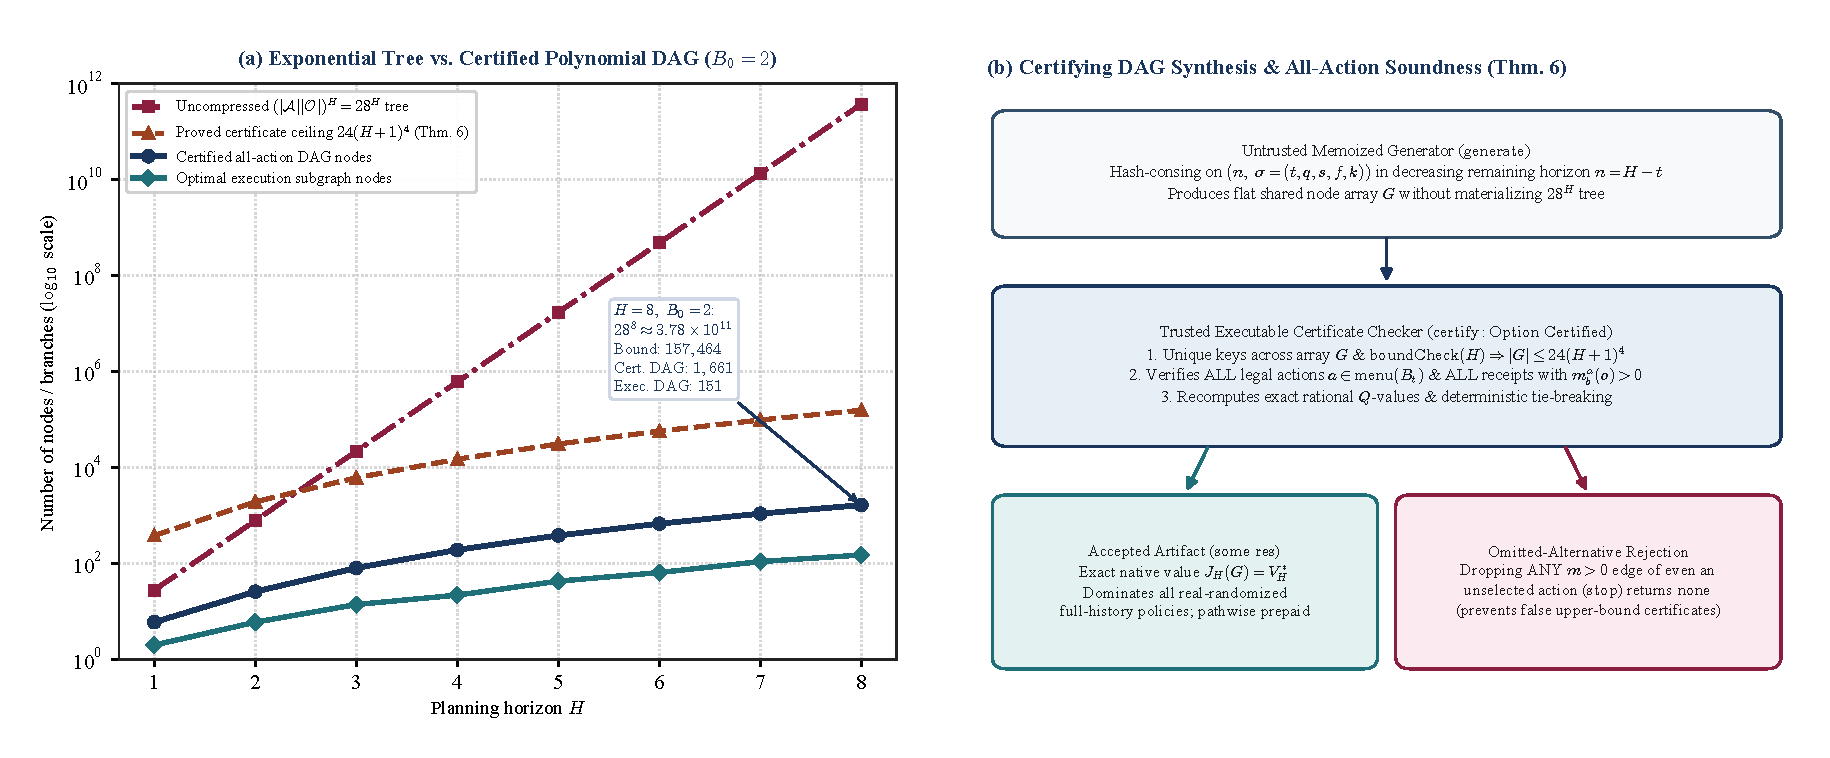
\includegraphics[width=0.99\linewidth,height=\textheight,keepaspectratio,alt={Exponential
history-tree explosion versus certified polynomial decision-diagram
scaling and two-stage certifying architecture (Theorem 6). (a)
Logarithmic scaling across H \textbackslash in \textbackslash\{1,
\textbackslash dots, 8\textbackslash\} at B\_0 = 2 comparing raw
(\textbar\textbackslash mathcal\{A\}\textbar\textbar\textbackslash
mathcal\{O\}\textbar)\^{}H = 28\^{}H trees against the proved
24(H+1)\^{}4 worst-case certificate ceiling, actual certified all-action
DAG nodes (1,661 at H=8), and optimal execution subgraph nodes (151 at
H=8). (b) Separation between the untrusted memoized DAG generator and
the executable rational certificate checker certify : Option Certified,
showing rejection when any positive-mass branch of an unselected
alternative action is
omitted.}]{figures/fig3_dag_compression_and_scaling.pdf}
\caption{Exponential history-tree explosion versus certified polynomial
decision-diagram scaling and two-stage certifying architecture (Theorem
6). (a) Logarithmic scaling across \(H \in \{1, \dots, 8\}\) at
\(B_0 = 2\) comparing raw \((|\mathcal{A}||\mathcal{O}|)^H = 28^H\)
trees against the proved \(24(H+1)^4\) worst-case certificate ceiling,
actual certified all-action DAG nodes (\(1,661\) at \(H=8\)), and
optimal execution subgraph nodes (\(151\) at \(H=8\)). (b) Separation
between the untrusted memoized DAG generator and the executable rational
certificate checker \protect\texttt{certify\ :\ Option\ Certified},
showing rejection when any positive-mass branch of an unselected
alternative action is omitted.}
\end{figure}

\section{Formalization architecture, related literature, and explicit
scope
boundaries}\label{formalization-architecture-related-literature-and-explicit-scope-boundaries}

\subsection{Pure-kernel Lean 4 formalization and exact rational
certificate
checking}\label{pure-kernel-lean-4-formalization-and-exact-rational-certificate-checking}

All definitions, recursions, posterior updates, witness trajectories,
and theorems in Sections 2--6 have been formalized in Lean 4 (v4.33.1)
over Mathlib \citep{mouraUllrich2021, mathlib2020} across 24
interconnected modules (\texttt{FiniteJointDecision*},
\texttt{RegisterJointDecision*}, and \texttt{RegisterDecision*}). Across
the entire compiled environment, an automated axiom audit confirms zero
occurrences of \texttt{sorryAx} and zero occurrences of compiler-trusted
evaluation (\texttt{Lean.ofReduceBool} / \texttt{native\_decide};
\citet{boespflug2011}), leaving solely Lean's three standard logical
axioms \texttt{\{propext,\ Classical.choice,\ Quot.sound\}}
\citep{carneiro2019}.

Architecturally, the formalization enforces three methodological
safeguards that complement prior mechanized developments in probability,
information theory, and Markov decision processes
\citep{nipkowPaulsonWenzel2002, bertotCasteran2004, affeldt2014, eberl2015, hoelzl2017, vajjha2021, schaeffelerAbdulaziz2023}
as well as probabilistic model checking
\citep{baierKatoen2008, kwiatkowska2011}:

\begin{enumerate}
\def\labelenumi{\arabic{enumi}.}
\tightlist
\item
  \textbf{Non-circular derivation of sufficiency
  (\texttt{initial\_relation} and \texttt{StepRefinement}).} Rather than
  axiomatizing a reduced state space \(\Sigma\) as primitive, the
  \texttt{RegisterDecision} modules \texttt{ObserverSource} and
  \texttt{RepresentationModel} construct an explicit world-level
  simulation relation \texttt{Rel} linking full finitely supported
  beliefs over \(\mathcal{W}(\Theta)\) to \(\sigma = (t, q, s, f, k)\),
  prove \texttt{initial\_relation} on the damaged founder
  \(\mathcal{S}_0\), and discharge \texttt{StepRefinement} for every
  legal action and positive-mass receipt.
\item
  \textbf{Separation between noncomputable real expectations and
  executable rational artifacts.} Native genealogical expectations
  (\texttt{nativeTotal}, \texttt{expectedRawNativeJ}) are formulated
  over \(\mathbb{R}\) and \texttt{PMF} to interface cleanly with general
  real-randomized competitors (\texttt{RawCausalPolicy}), whereas
  \texttt{summarize}, \texttt{countBelief}, \texttt{generate},
  \texttt{certify}, \texttt{boundCheck}, and \texttt{packedRun} execute
  purely over computable types (\texttt{ℕ}, \texttt{ℚ}, \texttt{Bool},
  \texttt{Option}, \texttt{Array}). Exact bridge theorems
  (\texttt{checked\_native\_value}, \texttt{checked\_native\_optimal},
  \texttt{initial\_graph\_native\_payment}) equate the two layers
  without runtime real arithmetic.
\item
  \textbf{Explicit \texttt{Option} certificate boundary
  (\texttt{certify\ :\ Option\ Certified}).} Theorem 6 proves soundness
  of \emph{every accepted graph} (\texttt{certify\ G\ =\ some\ res}),
  rather than claiming an unproved totality theorem that
  \texttt{generate} must pass \texttt{certify} on every conceivable
  input; separately, all five main benchmarks (Table 3) and eight
  boundary stress tests (\(H = 0\), \(B_0 = 0\), \(B_0 < c\), endpoint
  rates \(r \in \{0,1\}\), zero-weight prior atoms, duplicate rate
  atoms, and inverted target \(g = 0\)) are explicitly generated and
  accepted.
\end{enumerate}

\subsection{Comparison with classical operations research and explicit
scope
boundaries}\label{comparison-with-classical-operations-research-and-explicit-scope-boundaries}

Our results bridge several distinct literatures in stochastic control
and operations research:

\begin{itemize}
\tightlist
\item
  \textbf{Controlled branching vs.~partially observed maintenance.}
  Classical multitype branching optimization
  \citep{harris1963, sevastyanov1971, athreyaNey1972, pliska1976, rothblumWhittle1982, gonzalez2018}
  characterizes asymptotic Perron growth eigenvalues under full state
  observation and unconstrained per-step action sets, whereas partially
  observed maintenance and replacement
  \citep{eckles1968, ross1971, barlowProschan1975, white1979, monahan1982, makisJiang2003}
  studies single-unit wear without offspring generation. Our model
  unites regenerative standby creation (\texttt{child1}) with partial
  receipt observation and hard finite-wallet prepayment, showing how
  finite-horizon zero-terminal optimization differs qualitatively from
  infinite-horizon growth rate maximization.
\item
  \textbf{Bayesian adaptive control, bandits, and constrained MDPs.} In
  multi-armed bandits and Bayesian adaptive control
  \citep{robbins1952, bellman1961, rieder1975, gittins1979, whittle1982, easleyKiefer1988, aghion1991, duff2002, ross2011},
  actions trade immediate reward against parameter information, while
  risk-sensitive and constrained MDPs
  \citep{altman1999, feinberg2000, bauerleRieder2011, mannorTsitsiklis2013}
  or knapsack bandits \citep{besbesZeevi2009, badanidiyuru2018} impose
  resource limits. Theorem 3 reveals a striking asymmetry under hard
  prepayment: prior variance raises initial repair value
  (\(d\,\mathrm{Var}(r_\theta)\)) and fault receipts strictly contract
  retry thresholds (\(p_{\mathrm{fault}}^* < p_{\mathrm{prior}}^*\)),
  yet post-repair parameter learning has \emph{zero} value
  (\(\mathrm{EVPI}_{\mathrm{post}} = 0\)) even while post-repair
  \emph{body-state} receipt feedback has strictly positive value
  (\(d^3\mathbb{E}[r_\theta^3(1-r_\theta)]\)).
\item
  \textbf{Sufficient statistics and decision diagrams.} Whereas general
  POMDP belief spaces remain continuous
  \citep{smallwoodSondik1973, sondik1978, lovejoy1991, kaelbling1998}---motivating
  approximate information states \citep{subramanian2022} or bounded
  controllers \citep{hansen1998, poupartBoutilier2003}---Theorem 4 and
  Theorem 5 show that filtering out deterministic \((0,0)\) receipts
  yields an \emph{exact} discrete counting posterior across arbitrary
  randomized policies, compressing exponential trees into \(O(H^4)\)
  all-action certified DAGs
  \citep{bryant1986, bahar1997, hoey1999, bergman2016}.
\end{itemize}

At the same time, four scope boundaries must be stated explicitly:

\begin{enumerate}
\def\labelenumi{\arabic{enumi}.}
\tightlist
\item
  \emph{Node-count ceiling versus bit-complexity and runtime memory.}
  The bound \(N_H \le 24(H+1)^4\) bounds the number of stored rows in
  the certified array \(G\) for fixed dispatch slots
  \texttt{\{root0,\ child1\}}. It does not bound the bit-length of exact
  rational denominators \(Z(s,f)\) as \(H \to \infty\), the cardinality
  \(|\Theta|\), or total process memory, nor does it claim
  polynomial-time solvability for general POMDPs
  \citep{papadimitriouTsitsiklis1987, madani2003}. Furthermore, external
  computer time and memory spent solving or checking \(G\) lie outside
  the physical wallet \(B_0\).
\item
  \emph{Menu-relativity and known-target alignment.} Both compressed
  commutation (Theorem 1) and five-coordinate sufficiency (Theorem 5)
  rely on known public target alignment (\(\mathrm{prog} = g\)) and
  dispatch restricted to addresses \(\{0, 1\}\). As Theorem 5(3)
  demonstrates, granting dispatch access to slot \(2\) immediately
  requires refining \(\sigma\); unknown target programs, simultaneous
  whole-population aging, or correlated whole-store faults constitute
  distinct mathematical problems.
\item
  \emph{Finite-horizon zero-terminal contract versus infinite-horizon
  persistence.} Optimality here holds strictly for the pre-specified
  discounted net output \(J_H\) with zero terminal salvage value and
  zero external income, and should not be conflated with
  infinite-horizon survival or asymptotic lineage growth.
\end{enumerate}

\section{Appendix: Self-contained mathematical
proofs}\label{appendix-self-contained-mathematical-proofs}

\subsection{A.1 Proof of Theorem 1 (Commutation, prepayment, and
full-history Bayes
optimality)}\label{a.1-proof-of-theorem-1-commutation-prepayment-and-full-history-bayes-optimality}

\textbf{(1) Exact native-to-compressed commutation.} Proceed by
induction on \(t \in \{0, \dots, H\}\). At \(t = 0\),
\(\mathcal{S}_0 = [\mathrm{Some}(p_0)]\) has length \(L_0 = 1\),
\(\mathrm{prog}(p_0) = g\) so \(\mathrm{Aligned}(g, \mathcal{S}_0)\)
holds, and
\(\mathrm{project}(\mathcal{S}_0) = [\mathrm{Some}(\neg g)]\). Suppose
at step \(t\) that \(\mathrm{Aligned}(g, \mathcal{S}_t)\) holds,
\(L_t = 1 + t\), and \(s_t = \mathrm{project}(\mathcal{S}_t)\). Let
\((j_{\mathrm{eff}}, \alpha_{\mathrm{eff}}) = \mathrm{eff}(\mathrm{stopped}_t, a_t)\)
and \(z_t = (m_t, \ell_t) \in \{0,1\}^2\).

\begin{itemize}
\tightlist
\item
  \emph{Case 1: \(\mathcal{S}_t[j_{\mathrm{eff}}] = \mathrm{None}\) (or
  \(j_{\mathrm{eff}} \ge L_t\)).} By definition of \texttt{project},
  \(s_t[j_{\mathrm{eff}}] = \mathrm{None}\) as well. Both native and
  compressed transitions leave existing slots \(0, \dots, L_t - 1\)
  unchanged, append \texttt{None} at index \(L_t\) (so
  \(L_{t+1} = L_t + 1 = 1 + (t+1)\) and
  \(\mathrm{Aligned}(g, \mathcal{S}_{t+1})\) is preserved), emit receipt
  \(o_t = (0,0)\), and charge literal fee \(C_t = 0\).
\item
  \emph{Case 2: \(\mathcal{S}_t[j_{\mathrm{eff}}] = \mathrm{Some}(p)\)
  with physical bit \(x \in \{0,1\}\).} Then
  \(s_t[j_{\mathrm{eff}}] = \mathrm{Some}(x)\), and by
  \(\mathrm{Aligned}(g, \mathcal{S}_t)\), \(\mathrm{prog}(p) = g\). In
  the native transaction, the post-step parent organism \(p'\) at slot
  \(j_{\mathrm{eff}}\) retains \(\mathrm{prog}(p') = g\) and updates its
  physical bit to \(x' = x_{\mathrm{cand}}(x, \alpha_{\mathrm{eff}})\)
  if \(m_t = 1\) and \(\neg g\) if \(m_t = 0\), matching
  \(\mathrm{postBit}(g, x, \alpha_{\mathrm{eff}}, m_t)\). Because
  \(\mathrm{prog}(p) = g\), a newborn \(c_{\mathrm{new}}\) is created in
  the native transaction iff \(m_t = 1\) and
  \(x' = \mathrm{prog}(p) = g\), in which case
  \(\mathrm{phys}(c_{\mathrm{new}}) = g\) and
  \(\mathrm{prog}(c_{\mathrm{new}}) = g\), matching
  \(\mathrm{childBit}(g, x, \alpha_{\mathrm{eff}}, m_t) = \mathrm{Some}(g)\)
  and preserving \(\mathrm{Aligned}(g, \mathcal{S}_{t+1})\); otherwise
  \texttt{None} is appended in both stores. Thus
  \(\mathrm{project}(\mathcal{S}_{t+1}) = s_{t+1}\),
  \(L_{t+1} = L_t + 1\), and both receipt bits
  \((\mathrm{birth}_t, \mathrm{paid}_t) = (\mathbf{1}_{\{\mathrm{childBit} \neq \mathrm{None}\}},\, \mathbf{1}_{\{m_t = 1 \land \alpha_{\mathrm{eff}} \neq \mathrm{idle}\}})\)
  and literal fee \(C_t = c\,\mathrm{paid}_t\) agree identically.
\end{itemize}

\textbf{(2) Strict sample-path prepayment.} For every world \(w\),
action \(a \in \mathcal{A}\), and noise \(z = (m, \ell)\), inspect
\(\mathrm{paid}(w, a, z) \in \{0,1\}\)
vs.~\(\mathrm{cap}(a) \in \{0,1\}\): if
\(a \in \{\mathrm{stop}, (0,\mathrm{idle}), (1,\mathrm{idle})\}\), then
\(\alpha_{\mathrm{eff}} = \mathrm{idle}\), so
\(\mathrm{paid}(w,a,z) = 0 = \mathrm{cap}(a)\); if
\(a = (j, \mathrm{write}_v)\), then
\(\mathrm{cap}(a) = 1 \ge \mathrm{paid}(w,a,z)\) regardless of whether
\(w.\mathrm{stopped} = 1\), \(s[j] = \mathrm{None}\), or \(m = 0\).
Hence \(0 \le C_t = c\,\mathrm{paid}_t \le c\,\mathrm{cap}(a_t)\) holds
pathwise. On any prefix \(h_t\) of strictly positive probability under a
supported-admissible policy \(\pi\), every prefix \(h_s\) (\(s < t\))
also has strictly positive probability and \(\pi_s(h_s)(a_s) > 0\), so
\(a_s \in \mathrm{menu}(c, B_s)\), meaning
\(c\,\mathrm{cap}(a_s) \le B_s\). By induction on \(s = 0, \dots, t\):
\(B_0 \ge 0\), and if \(B_s = B_0 - \sum_{u < s} C_u \ge 0\), then
\(B_s - C_s \ge B_s - c\,\mathrm{cap}(a_s) \ge 0\), so
\(\max\{0, B_s - C_s\} = B_s - C_s = B_0 - \sum_{u \le s} C_u \ge 0\).

\textbf{(3) Attainment and optimality over real-randomized full-history
policies.} By Part (1), for every fixed \((\theta, z_{0:H-1})\) and
action sequence \(a_{0:H-1}\), native discounted net payoff equals
compressed discounted net payoff, so
\(J_H^{\mathrm{native}}(\pi) = J_H^{\mathrm{comp}}(\pi)\) for every
real-randomized history policy \(\pi\). Let
\(h_t \in (\mathcal{A} \times \mathcal{O})^t\) be any prefix with
\(\mathbb{P}_{\pi_0, \pi}(h_t) > 0\). Because \(K_{w.\theta}(z_s)\) and
transitions \(T, O\) do not depend on \(\pi\), the conditional
distribution over \(\mathcal{W}(\Theta)\) given \(h_t\) equals the
deterministic recursively filtered belief \(b(h_t)\) (starting from
\(b([]) = b_0\), since along \(h_t\) each step receipt satisfies
\(m_{b(h_s)}^{a_s}(o_s) > 0\)), and the remaining balance is
\(B(h_t) \ge 0\) by Part (2). Prove by backward induction on remaining
steps \(n = H - t \in \{0, \dots, H\}\) that for every
supported-admissible \(\pi\) and every prefix \(h_t\) with
\(\mathbb{P}_{\pi_0, \pi}(h_t) > 0\), the conditional expected
continuation payoff \(J_n(\pi \mid h_t)\) satisfies
\(J_n(\pi \mid h_t) \le V_n(b(h_t), B(h_t))\), with equality when
\(\pi = \tau_H^*\). At \(n = 0\), \(0 \le 0\). From \(n\) to \(n+1\)
(\(t = H - 1 - n\)): since \(\mathbb{P}_{\pi_0, \pi}(h_t) > 0\) and
\(\pi\) is supported-admissible, every \(a \in \mathcal{A}\) with
\(\pi_t(h_t)(a) > 0\) lies in \(\mathrm{menu}(c, B(h_t))\), and for
every \(o \in \mathcal{O}\) with \(m_{b(h_t)}^a(o) > 0\), the extended
prefix \(h_{t+1} = h_t \mathbin{+\!+} [(a,o)]\) has
\(\mathbb{P}_{\pi_0, \pi}(h_{t+1}) = \mathbb{P}_{\pi_0, \pi}(h_t)\,\pi_t(h_t)(a)\,m_{b(h_t)}^a(o) > 0\),
so by the induction hypothesis
\(J_n(\pi \mid h_{t+1}) \le V_n(b(h_t)^{a,o}, B(h_t) - c\mathbf{1}_{\{o_2=1\}})\).
Taking the convex combination over \(a \sim \pi_t(h_t)\):
\[\begin{aligned}
J_{n+1}(\pi \mid h_t)
&= \sum_{a : \pi_t(h_t)(a) > 0} \pi_t(h_t)(a) \sum_{o : m_{b(h_t)}^a(o) > 0} m_{b(h_t)}^a(o)\Bigl[R(o) + d\, J_n\bigl(\pi \mid h_t \mathbin{+\!+} [(a,o)]\bigr)\Bigr] \\
&\le \sum_{a : \pi_t(h_t)(a) > 0} \pi_t(h_t)(a) \max_{a' \in \mathrm{menu}(c, B(h_t))} Q_{n+1}\bigl(b(h_t), B(h_t), a'\bigr) = V_{n+1}\bigl(b(h_t), B(h_t)\bigr),
\end{aligned}\] where
\(R(o) = \mathbf{1}_{\{o_1=1\}} - \lambda c \mathbf{1}_{\{o_2=1\}}\),
and \(\tau_H^*\) achieves equality at every \(n\) by deterministically
choosing the canonical maximizer \(a^* \in \mathrm{menu}(c, B(h_t))\) on
every branch. Evaluating at \(t = 0\) (\(h_0 = []\), probability \(1\))
gives
\(J_H^{\mathrm{native}}(\pi) \le V_H(b_0, B_0) = J_H^{\mathrm{native}}(\tau_H^*)\).
\(\square\)

\subsection{A.2 Proof of Theorem 2 (High-price closed-form optimum and
sharp
boundaries)}\label{a.2-proof-of-theorem-2-high-price-closed-form-optimum-and-sharp-boundaries}

\textbf{(1) Universal impossibility when \(B_0 < c\).} If \(B_0 < c\),
then for every \(B \in [0, B_0]\),
\(\mathrm{menu}(c, B) = \{\mathrm{stop}, (0, \mathrm{idle}), (1, \mathrm{idle})\}\)
contains zero write actions (\texttt{cap} \(= 1\) requires \(c \le B\)).
Starting from \(\mathcal{S}_0 = [\mathrm{Some}(\neg g)]\), idling slot
\(0\) (\(\neg g\)) produces post-bit \(\neg g\) under both \(m = 1\) and
\(m = 0\), emits no child (\texttt{None} appended at slot \(1\) and all
later slots), and charges \(C_t = 0\); idling slot \(1\) (\texttt{None})
likewise emits \((0,0)\) and charges \(0\). By induction on \(t\), on
every positive-probability trajectory under any supported-admissible
\(\pi\), \(\mathrm{birth}_t = 0\) and \(C_t = 0\) for all \(t < H\), so
\(J_H^{\mathrm{native}}(\pi) = 0\).

\textbf{(2) Two-object continuation upper bound and attainment at
\(B = 0\).} Fix reliability \(r \in [0,1]\) and exhausted balance
\(B = 0\), so only \texttt{stop}, \((0, \mathrm{idle})\), and
\((1, \mathrm{idle})\) are legal. For any compressed store \(s\), let
\(\nu(s) \in \{0, 1, 2\}\) count how many of the two dispatchable slots
\(\{0, 1\}\) currently hold \(\mathrm{Some}(g)\). Because zero-fee
actions never write \(g\) and never fill slot \(1\) once \(t \ge 1\),
\(\nu(s)\) is nonincreasing along every step: - If \(\nu(s) = 0\), every
legal action yields \(\mathrm{birth} = 0\) and \(\nu(s') = 0\), so
continuation payoff is \(0\). - By induction on remaining steps
\(n \ge 0\), prove that any state \(s\) with \(\nu(s) \le 1\) has
optimal zero-write continuation bounded above by \(U_1(r, d, n)\), and
any state \(s\) with \(\nu(s) \le 2\) has continuation bounded above by
\(U_2(r, d, n) \ge U_1(r, d, n)\) (noting
\(U_2(r,d,n) - U_1(r,d,n) \ge 0\) easily by induction:
\(U_2(r,d,n+1) - U_1(r,d,n+1) = r d(U_2 - U_1) + (1-r)d U_1 \ge 0\)): -
When \(\nu(s) = 1\), because \(U_1(r, d, m)\) is nondecreasing in \(m\)
(\(U_1(r,d,0) = 0 \le r = U_1(r,d,1)\) and
\(U_1(m+1) - U_1(m) = d r (U_1(m) - U_1(m-1)) \ge 0\)) and
\(d \in [0,1]\), dispatching the damaged or absent slot yields
continuation value bounded above by
\(0 + d\,U_1(r, d, n-1) \le U_1(r, d, n-1) \le U_1(r, d, n) = r(1 + d\,U_1(r, d, n-1))\),
whereas idling the unique intact slot attains
\(r(1 + d\,U_1(r, d, n-1)) + (1 - r)\cdot 0 = U_1(r, d, n)\). - When
\(\nu(s) = 2\) (both \texttt{root0} and \texttt{child1} hold \(g\)),
\texttt{stop} commits to \((0, \mathrm{idle})\) forever (attaining
\(U_1(r, d, n) \le U_2(r, d, n)\)), while idling either intact slot
yields
\(r(1 + d\,\text{cont}_{\nu=2}) + (1-r)(0 + d\,\text{cont}_{\nu=1}) \le r(1 + d U_2(r, d, n-1)) + (1-r) d U_1(r, d, n-1) = U_2(r, d, n)\).
Conversely, \texttt{freeSchedule}---which idles \texttt{root0} while
receipts equal \((1,0)\) and switches permanently to
\((1, \mathrm{idle})\) upon the first \((0,0)\) receipt---uses only
delivered receipts and attains \(U_2(r, d, n)\) identically for every
\(r \in [0,1]\).

\textbf{(3) Five-step proof of the general high-price formula
(\(B_0 = c\), \(p \ge S_H(d)\)).} Fix \(\theta \in \Theta\) with rate
\(r = r_\theta\) and total horizon \(H + 1\). 1. \emph{Delayed-charge
pathwise nonpositivity.} On any legal trajectory starting from
\(\mathcal{S}_0 = [\mathrm{Some}(\neg g)]\), let
\(\tau \in \{0, 1, \dots, H\} \cup \{\infty\}\) be the first step at
which a paid write occurs (\(\mathrm{paid}_\tau = 1\), \(C_\tau = c\)).
For all \(t < \tau\), either no write was requested or the write faulted
(\(m_t = 0\)) or targeted absent slot \(1\), so all slots remain
\(\neg g\) or \texttt{None} and \(\mathrm{birth}_t = 0\). If
\(\tau = \infty\), pathwise payoff is \(0\). If \(1 \le \tau \le H\),
since \(\mathrm{birth}_t \le 1\) for \(t \ge \tau\) and \(C_t \ge 0\)
for \(t > \tau\), total pathwise discounted net payoff is bounded above
by
\[\sum_{t=\tau}^{H} d^t \mathrm{birth}_t - d^\tau \lambda c \le d^\tau \sum_{u=0}^{H-\tau} d^u - d^\tau p = d^\tau\bigl(S_{H-\tau+1}(d) - p\bigr) \le d^\tau\bigl(S_H(d) - p\bigr) \le 0,\]
because
\(\tau \ge 1 \implies H - \tau + 1 \le H \implies S_{H-\tau+1}(d) \le S_H(d) \le p\).
2. \emph{Suboptimality of non-repair initial actions.} Any initial
action \(a_0 \neq (0, \mathrm{write}_g)\)---namely \texttt{stop},
\((0, \mathrm{idle})\), \((1, \mathrm{idle})\),
\((0, \mathrm{write}_{\neg g})\), or \((1, \mathrm{write}_v)\) on absent
slot \(1\)---produces \(\mathrm{birth}_0 = 0\), nonpositive immediate
reward \(-\lambda C_0 \le 0\), and leaves an all-damaged store at
\(t = 1\) with remaining horizon \(H\). Every subsequent realization
then either never pays a write fee (0 births) or pays its first
remaining write fee at step \(t \ge 1\), giving total pathwise payoff
\(\le 0\) by Step 1. 3. \emph{Exact conditional decomposition of initial
\((0, \mathrm{write}_g)\).} Submitting \(a_0 = (0, \mathrm{write}_g)\)
faults w.p. \(1 - r\) (emitting \((0,0)\), charging \(0\), and leaving
\(\mathcal{S}_1 = [\mathrm{Some}(\neg g), \mathrm{None}]\) with
remaining horizon \(H\), where every legal continuation has conditional
expected value \(\le 0\) by Step 1, and \texttt{stop} attains \(0\));
and succeeds w.p. \(r\) (emitting \((1,1)\), earning immediate net
reward \(1 - p\), producing intact \texttt{root0} and \texttt{child1}
with \(\nu = 2\), and exhausting wallet \(B_1 = c - c = 0\)). 4.
\emph{Post-repair zero-wallet upper bound.} On the \((1,1)\) branch
(\(B_1 = 0\), \(H\) steps left), Part (2) proves that every legal
continuation has conditional expected value at most \(U_2(r, d, H)\),
attained uniformly by \texttt{freeSchedule}. 5. \emph{Prior expectation
and attainment.} Averaging over \(\theta \sim \pi_0\) shows that every
supported-admissible real-randomized policy \(\pi\) satisfies
\(J_{H+1}(\pi) \le \max\{0,\, \mathbb{E}_{\pi_0}[r_\theta(1 - p + d\,U_2(r_\theta, d, H))]\}\),
while choosing \((0, \mathrm{write}_g)\) followed by
\texttt{freeSchedule} on \((1,1)\) and \texttt{stop} on \((0,0)\)
attains
\(\mathbb{E}_{\pi_0}[r_\theta(1 - p + d\,U_2(r_\theta, d, H))]\), and
\texttt{stop} at \(t = 0\) attains \(0\). Finally, for
\(\mu_1 = \mathbb{E}[r_\theta] > 0\),
\(\mathbb{E}[r_\theta(1 - p + d U_2(r_\theta, d, H))] = \mu_1(1 - p) + d M_H > 0 \iff p < 1 + d M_H / \mu_1\).
\(\square\)

\subsection{A.3 Proof of Theorem 3 (Persistence, post-fault contraction,
feedback, and zero
EVPI)}\label{a.3-proof-of-theorem-3-persistence-post-fault-contraction-feedback-and-zero-evpi}

\textbf{(1) Persistence variance premium.} At \(H = 1\) (total horizon
\(2\)), Theorem 2 gives
\(V_{2,\mathrm{repair}} = \mathbb{E}[r_\theta(1 - p + d r_\theta)] = \mu_1(1 - p) + d\mu_2\).
Under stepwise i.i.d. redrawing \(\theta_0, \theta_1 \sim \pi_0\),
step-\(0\) success has probability \(\mu_1\) and independent step-\(1\)
birth has probability \(\mu_1\), giving \(\mu_1(1 - p) + d\mu_1^2\);
subtracting yields
\(d(\mu_2 - \mu_1^2) = d\,\mathrm{Var}(r_\theta) \ge 0\). For
\(r \in \{1/4, 3/4\}\) equally weighted, \(\mu_1 = 1/2\) and
\(\mu_2 = \frac{1}{2}(\frac{1}{16} + \frac{9}{16}) = \frac{5}{16}\); at
\(d = 1/2, p = 13/10 \ge 1\),
\(\mu_1(1-p) + d\mu_2 = \frac{1}{2}(-\frac{3}{10}) + \frac{5}{32} = -\frac{3}{20} + \frac{5}{32} = \frac{-24 + 25}{160} = \frac{1}{160}\),
whereas
\(\mu_1(1-p) + d\mu_1^2 = -\frac{3}{20} + \frac{1}{8} = -\frac{1}{40}\).

\textbf{(2) Post-fault threshold contraction.} After
\(a_0 = (0, \mathrm{write}_g)\), \(o_0 = (0,0)\) occurs iff \(m_0 = 0\),
which has conditional likelihood \(1 - r_\theta\) and prior mass
\(1 - \mu_1 > 0\). Thus
\(\pi_{(0,0)}(\theta) = \pi_0(\theta)(1 - r_\theta)/(1 - \mu_1)\) and
\(\mu'_k = \sum_\theta r_\theta^k \pi_{(0,0)}(\theta) = (\mu_k - \mu_{k+1})/(1 - \mu_1)\).
For a two-point prior \(w \delta_{r_0} + (1-w)\delta_{r_1}\) with
\(w \in (0,1)\) and \(0 < r_0 < r_1 < 1\), expand directly:
\[\begin{aligned}
\mu_1 \mu_3 - \mu_2^2
&= \bigl(w r_0 + (1-w)r_1\bigr)\bigl(w r_0^3 + (1-w)r_1^3\bigr) - \bigl(w r_0^2 + (1-w)r_1^2\bigr)^2 \\
&= w(1-w)\bigl(r_0 r_1^3 + r_1 r_0^3 - 2 r_0^2 r_1^2\bigr)
= w(1-w) r_0 r_1 (r_0 - r_1)^2 > 0.
\end{aligned}\] Since \(0 < r_0 < r_1 < 1\), we also have
\(\mu_1 > \mu_2 > 0\), so
\[\frac{\mu_2}{\mu_1} - \frac{\mu_2 - \mu_3}{\mu_1 - \mu_2}
= \frac{\mu_2(\mu_1 - \mu_2) - \mu_1(\mu_2 - \mu_3)}{\mu_1(\mu_1 - \mu_2)}
= \frac{\mu_1 \mu_3 - \mu_2^2}{\mu_1(\mu_1 - \mu_2)} > 0,\] proving
\(p_{\mathrm{fault}}^*(1) = 1 + d\frac{\mu_2 - \mu_3}{\mu_1 - \mu_2} < 1 + d\frac{\mu_2}{\mu_1} = p_{\mathrm{prior}}^*(1)\)
whenever \(d > 0\). For \(w = 1/2, (r_0, r_1) = (1/4, 3/4), d = 1/2\):
\(\mu_1 = 1/2, \mu_2 = 5/16, \mu_3 = \frac{1}{2}(\frac{1}{64} + \frac{27}{64}) = \frac{7}{32}\),
so
\(p_{\mathrm{prior}}^*(1) = 1 + \frac{1}{2}\cdot\frac{5/16}{1/2} = \frac{21}{16}\)
and
\(p_{\mathrm{fault}}^*(1) = 1 + \frac{1}{2}\cdot\frac{5/16 - 7/32}{1/2 - 5/16} = 1 + \frac{1}{2}\cdot\frac{3/32}{3/16} = \frac{5}{4}\).
At \(p = 13/10\), the conditional post-fault two-step retry value is
\(\mu'_1(1-p) + d\mu'_2 = \frac{3}{8}(-\frac{3}{10}) + \frac{1}{2}\cdot\frac{3}{16} = -\frac{9}{80} + \frac{3}{32} = -\frac{3}{160} < 0\).
Hence at total horizon \(3\) (\(d = 1/2, p = 13/10\)), after
\(a_0 = (0, \mathrm{write}_g)\): the \((1,1)\) branch contributes
\(\mu_1(1 - 13/10) + (1/2 + 1/4)\mu_2 = -\frac{3}{20} + \frac{3}{4}\cdot\frac{5}{16} = \frac{27}{320}\),
and halting after \((0,0)\) contributes \(0\) (\(V_3^* = 27/320\)),
whereas freezing the prior and retrying \((0, \mathrm{write}_g)\) after
\((0,0)\) (branch probability \(1 - \mu_1 = 1/2\), discounted by
\(d = 1/2\)) adds
\((1 - \mu_1) d \bigl(\mu'_1(1-p) + d\mu'_2\bigr) = \frac{1}{2}\cdot\frac{1}{2}\cdot\bigl(-\frac{3}{160}\bigr) = -\frac{3}{640}\),
reducing total expected net value to
\(\frac{27}{320} - \frac{3}{640} = \frac{51}{640}\).

\textbf{(3) Three-step backup, four-step feedback, and (4) zero
post-repair EVPI.} At \(H+1 = 3\), fixed sequence
\([(0, \mathrm{write}_g), (0, \mathrm{idle}), (1, \mathrm{idle})]\)
earns \(1 - p + d\mathbf{1}_{\{m_1=1\}} + d^2\mathbf{1}_{\{m_2=1\}}\)
whenever \(m_0 = 1\) (since step \(1\) touches only \texttt{root0},
leaving \texttt{child1} intact for step \(2\) regardless of \(m_1\)),
whose expectation is \(\mu_1(1-p) + (d + d^2)\mu_2\); at
\(r \in \{1/4, 3/4\}, d = 3/4, p = 7/4\),
\(\frac{1}{2}(-\frac{3}{4}) + (\frac{3}{4} + \frac{9}{16})\frac{5}{16} = -\frac{3}{8} + \frac{21}{16}\cdot\frac{5}{16} = \frac{-96 + 105}{256} = \frac{9}{256}\),
whereas root-only
\([(0,\mathrm{write}_g),(0,\mathrm{idle}),(0,\mathrm{idle})]\) earns
\(\mu_1(1-p) + d\mu_2 + d^2\mu_3 = -\frac{3}{8} + \frac{3}{4}\cdot\frac{5}{16} + \frac{9}{16}\cdot\frac{7}{32} = \frac{-192 + 120 + 63}{512} = -\frac{9}{512}\).

At \(H+1 = 4\), after \(m_0 = 1\) creates two intact slots \(\{0, 1\}\),
consider any predetermined three-step open-loop sequence
\((j_1, j_2, j_3) \in \{0, 1\}^3\) of idles: - If \(j_1 = j_2 = j_3\):
expected continuation is \(r + d r^2 + d^2 r^3 \le r + d r + d^2 r^2\).
- If two consecutive steps use one slot and one step uses the
other---either \((0,0,1)\) (\(r + d r^2 + d^2 r\)) or \((0,1,1)\)
(\(r + d r + d^2 r^2\))---since
\(d r^2 + d^2 r - (d r + d^2 r^2) = d r(1-r)(d - 1) \le 0\) for
\(d \in [0,1]\), both are bounded above by \(r + d r + d^2 r^2\). - If
the sequence alternates \((0, 1, 0)\) (or \((1, 0, 1)\)): step \(1\)
earns \(r\), step \(2\) on the untouched slot earns \(d r\), and step
\(3\) returns to the first slot (which survived step \(1\) w.p. \(r\)
and succeeds at step \(3\) w.p. \(r\)), earning \(d^2 r^2\), totaling
\(r + d r + d^2 r^2\). By contrast, \texttt{freeSchedule} earns
\(U_2(r, d, 3) = r + d r + d^2(2r^2 - r^3)\), so multiplying by \(r d\)
and subtracting gives
\(r d\bigl(U_2(r,d,3) - (r + dr + d^2 r^2)\bigr) = d^3 r^3(1 - r) \ge 0\),
with expectation \(d^3 \mathbb{E}[r_\theta^3(1 - r_\theta)]\). For
\(r \in \{3/4, 7/8\}\) equally weighted,
\(d = 3/4, p = 37/16 \ge 1 + 3/4 + 9/16 = 37/16\): \(\mu_1 = 13/16\),
\(\mu_2 = \frac{1}{2}(\frac{9}{16} + \frac{49}{64}) = \frac{85}{128}\),
\(\mu_3 = \frac{1}{2}(\frac{27}{64} + \frac{343}{512}) = \frac{559}{1024}\),
\(\mu_4 = \frac{1}{2}(\frac{81}{256} + \frac{2401}{4096}) = \frac{3697}{8192}\).
Thus
\(V_{4,\mathrm{open}}^* = \frac{13}{16}(-\frac{21}{16}) + \frac{21}{16}\cdot\frac{85}{128} + \frac{27}{64}\cdot\frac{559}{1024} = \frac{2325}{65536} > 0\),
\(\Delta^{(4)} = \frac{27}{64}(\frac{559}{1024} - \frac{3697}{8192}) = \frac{27}{64}\cdot\frac{775}{8192} = \frac{20925}{524288}\),
and
\(V_4^* = \frac{2325}{65536} + \frac{20925}{524288} = \frac{39525}{524288}\).
Finally, Part (4) follows immediately from Appendix A.2(2): even if
\(\theta\) is revealed at \(t = 1\) when \(B_1 = 0\), no policy
depending on \(\theta\) can exceed \(U_2(r_\theta, d, H)\), which
\texttt{freeSchedule} already attains without knowing \(\theta\).
\(\square\)

\subsection{A.4 Proof of Theorem 4 (Informative zero receipts and
counting
posteriors)}\label{a.4-proof-of-theorem-4-informative-zero-receipts-and-counting-posteriors}

First verify the single-step likelihood factorization
\(L_r(o \mid g, q, a) = \mathbf{1}_{\{\mathrm{compatible}(g,q,a,o)\}} r^{\Delta s}(1-r)^{\Delta f}\)
across all \(r \in [0,1]\) (with \(0^0 = 1\)): - If
\(\mathrm{informative}(g, q, a)\) fails, then
\(o_{\mathrm{norm}}(g, q, a) = (0,0)\) and \(\Delta s = \Delta f = 0\).
If \(o = (0,0)\), compatibility holds and
\(L_r((0,0) \mid g, q, a) = r + (1 - r) = 1 = r^0 (1 - r)^0\) (even at
\(r = 0\) or \(r = 1\) since \(0^0 = 1\)); if \(o \neq (0,0)\),
compatibility fails and \(L_r(o \mid g, q, a) = 0\). - If
\(\mathrm{informative}(g, q, a)\) holds, then
\(o_{\mathrm{norm}} \neq (0,0)\). For \(o = o_{\mathrm{norm}}\),
\((\Delta s, \Delta f) = (1, 0)\) and \(L_r = r = r^1 (1 - r)^0\); for
\(o = (0,0)\), \((\Delta s, \Delta f) = (0, 1)\) and
\(L_r = 1 - r = r^0 (1 - r)^1\); for
\(o \notin \{o_{\mathrm{norm}}, (0,0)\}\), compatibility fails and
\(L_r = 0\).

Next, prove by induction along any step \(u\) from \(\mathcal{S}_0\)
that \texttt{upd}\((g, q_u, a_u, o_u)\) equals the local projection
\texttt{(s{[}0{]},\ s{[}1{]}?,\ stopped,\ L\ ==\ 1)} of the compressed
world \(w_{u+1}\) on every noise realization \(z_u\) emitting \(o_u\):
at \(u = 0\), \(q_0 = (\neg g, \mathrm{None}, 0, 1)\) matches
\([\mathrm{Some}(\neg g)]\) (\(L_0 = 1\)), and the \(u=0\) append sets
slot \(1\) to \(\mathrm{Some}(g)\) iff \(o_{0,1} = 1\) and \texttt{None}
iff \(o_{0,1} = 0\), setting \texttt{fresh} \(= 0\) (\(L_1 = 2\)); for
\(u \ge 1\) (\texttt{fresh} \(= 0\)), slot \(1\) is never overwritten if
\texttt{None}, and any existing dispatched slot
\(j_{\mathrm{eff}} \in \{0,1\}\) has post-bit \(g\) iff \(o_{u,1} = 1\)
and \(\neg g\) iff \(o_{u,1} = 0\). Summing
\(K_\theta(m_u, \ell_u) = \frac{1}{2}(r_\theta \mathbf{1}_{m_u=1} + (1-r_\theta)\mathbf{1}_{m_u=0})\)
over \(\ell_u \in \{0,1\}\) therefore gives the exact one-step receipt
probability \(L_{r_\theta}(o_u \mid g, q_u, a_u)\) independent of hidden
labels and tail slots \(j \ge 2\).

Now let \(\pi\) be any causal real-randomized policy (possibly seeded by
an initial private memory distribution \(\nu_0\) independent of
\(\theta\)). Conditional on \(\theta\) and private seed \(\zeta\), at
each step \(u < t\), \(\pi\)'s action probability
\(\pi_u(\zeta, h_u)(a_u)\) depends only on \((\zeta, h_u)\), never on
\(\theta\). Multiplying over \(u = 0, \dots, t-1\) and integrating over
\(\zeta \sim \nu_0\) defines
\(\alpha_\pi(h) := \int \prod_{u=0}^{t-1} \pi_u(\zeta, h_u)(a_u)\, d\nu_0(\zeta) \ge 0\),
which is completely independent of \(\theta\), while the environment
likelihood telescopes to
\(\prod_{u=0}^{t-1} L_{r_\theta}(o_u \mid g, q_u, a_u) = \mathbf{1}_{\{\mathrm{compat}(h)\}} r_\theta^{\sum_u \Delta s_u} (1 - r_\theta)^{\sum_u \Delta f_u} = \mathbf{1}_{\{\mathrm{compat}(h)\}} r_\theta^{s(h)} (1 - r_\theta)^{f(h)}\).
Multiplying by \(\pi_0(\theta)\) establishes Part (1). Summing over
\(\theta \in \Theta\) gives
\(\mathbb{P}_{\pi_0, \pi}(h) = \alpha_\pi(h) \mathbf{1}_{\{\mathrm{compat}(h)\}} Z(s(h), f(h))\);
thus \(\mathbb{P}_{\pi_0, \pi}(h) > 0\) implies \(\mathrm{compat}(h)\),
\(\alpha_\pi(h) > 0\), and \(Z(s(h), f(h)) > 0\), so
\(\mathbb{P}_{\pi_0, \pi}(\theta \mid h) = \mathbb{P}_{\pi_0, \pi}(\theta, h) / \mathbb{P}_{\pi_0, \pi}(h) = w_\theta(s(h), f(h)) / Z(s(h), f(h))\).
\(\square\)

\subsection{A.5 Proof of Theorem 5 (Joint all-action sufficiency and
sharpness
witnesses)}\label{a.5-proof-of-theorem-5-joint-all-action-sufficiency-and-sharpness-witnesses}

\textbf{(1) Joint sufficiency.} Let \(h\) be any positive-mass history
with \(\sigma(h) = (t, q, s, f, k)\). By Theorem 1(2), literal balance
is \(B(h) = B_0 - kc \ge 0\), determining \(\mathrm{menu}(c, B(h))\)
purely from \(k\). By Appendix A.4 and Theorem 4, every world
\(w = (\theta, s_{\mathrm{store}}, \mathrm{stopped})\) in the support of
\(b(h)\) projects locally to \(q\), and the \(\Theta\)-marginal of
\(b(h)\) equals \(\pi_{s,f}(\theta) = w_\theta(s,f)/Z(s,f)\) with
\(Z(s,f) > 0\). For any \(a \in \mathrm{menu}(c, B(h))\) and
\(o \in \mathcal{O}\), the marginal receipt probability under \(b(h)\)
is
\(m_{b(h)}^a(o) = \sum_{\theta \in \Theta} \pi_{s,f}(\theta)\, L_{r_\theta}(o \mid g, q, a)\),
while \(\sigma' = \mathrm{updStat}(g, \sigma, a, o)\),
\(\mathrm{birth} = \mathbf{1}_{\{o_1=1\}}\),
\(C = c\mathbf{1}_{\{o_2=1\}}\), and
\(B' = B_0 - (k + \mathbf{1}_{\{o_2=1\}})c\) are deterministic functions
of \((\sigma, a, o)\). Thus the joint law of
\((o, \sigma', \mathrm{birth}, C, B')\) depends \emph{only} on
\((\sigma, a)\). By backward induction on remaining steps \(n = H - t\),
the summary Bellman value \(V_n^{\mathrm{stat}}(\sigma)\) equals
\(V_n(b(h), B(h))\) for every positive-mass \(h\), matching
\(V_H^*(b_0, B_0)\) at \(t = 0\).

\textbf{(2) Physical-Markov insufficiency (\texttt{insufficientA}
vs.~\texttt{insufficientB}).} Under
\(a_{0:2} = [(0,\mathrm{write}_g), (0,\mathrm{idle}), (0,\mathrm{idle})]\)
starting from \([\mathrm{Some}(\neg g)]\): - History \(h_A\) emits
\([(1,1), (1,0), (0,0)]\), occurring iff
\((m_0, m_1, m_2) = (1, 1, 0)\), so \(\mathbb{P}_r(h_A) = r^2(1-r)\),
ending at \(t=3, k=1\) (\(B_3 = 0\)),
\(q_* = (\neg g, \mathrm{Some}(g), 0, 0)\), and \((s,f) = (2,1)\). Under
equal prior on \(\{1/4, 3/4\}\),
\(\mathbb{P}(h_A) = \frac{1}{2}\bigl(\frac{1}{16}\cdot\frac{3}{4} + \frac{9}{16}\cdot\frac{1}{4}\bigr) = \frac{12}{128} = \frac{3}{32}\),
\(\pi_{h_A}(1/4) = \frac{3/64}{12/64} = \frac{1}{4}\), and
\(\mathbb{P}(\mathrm{birth}_3 = 1 \mid h_A, a_3 = (1,\mathrm{idle})) = \frac{1}{4}\cdot\frac{1}{4} + \frac{3}{4}\cdot\frac{3}{4} = \frac{10}{16} = \frac{5}{8}\).
- History \(h_B\) emits \([(1,1), (0,0), (0,0)]\), occurring iff
\((m_0, m_1) = (1, 0)\) \emph{for both \(m_2 = 1\) and \(m_2 = 0\)}
(since after \(m_1 = 0\) damages \texttt{root0}, step \(2\) idles
damaged \texttt{root0} and emits \((0,0)\) deterministically), so
\(\mathbb{P}_r(h_B) = r(1-r)(r + 1 - r) = r(1-r)\), ending at the
\emph{same} \(t=3, B_3=0, q_*\), but \((s,f) = (1,1)\). Thus
\(\mathbb{P}(h_B) = \frac{1}{2}\bigl(\frac{3}{16} + \frac{3}{16}\bigr) = \frac{3}{16}\),
\(\pi_{h_B}(1/4) = \frac{1}{2}\), and
\(\mathbb{P}(\mathrm{birth}_3 = 1 \mid h_B, a_3 = (1,\mathrm{idle})) = \frac{1}{2}\cdot\frac{1}{4} + \frac{1}{2}\cdot\frac{3}{4} = \frac{1}{2} \neq \frac{5}{8}\).

\textbf{(3) Lawful history merger and slot-2 separation (\texttt{mergeA}
vs.~\texttt{mergeB}).} Under trajectory \(m_A\)
(\([(0,\mathrm{write}_g), (0,\mathrm{idle}), (1,\mathrm{idle})]\) with
\((m_0,m_1,m_2) = (1,0,1)\) and receipts \([(1,1),(0,0),(1,0)]\)), step
\(0\) appends \texttt{child1} at slot \(1\), step \(1\) faults on
\texttt{root0} appending \texttt{None} at slot \(2\), and step \(2\)
idles \texttt{child1} appending a grandchild at slot \(3\), giving
compressed store
\(s(m_A) = [\mathrm{Some}(\neg g), \mathrm{Some}(g), \mathrm{None}, \mathrm{Some}(g)]\).
Under trajectory \(m_B\)
(\([(0,\mathrm{write}_g), (1,\mathrm{idle}), (0,\mathrm{idle})]\) with
\((m_0,m_1,m_2) = (1,1,0)\) and receipts \([(1,1),(1,0),(0,0)]\)), step
\(1\) appends a grandchild at slot \(2\) and step \(2\) faults on
\texttt{root0} appending \texttt{None} at slot \(3\), giving compressed
store
\(s(m_B) = [\mathrm{Some}(\neg g), \mathrm{Some}(g), \mathrm{Some}(g), \mathrm{None}]\).
Both have likelihood \(r^2(1-r)\) (prior mass \(3/32\),
\(\pi(1/4) = 1/4\)) and identical summary
\(\sigma = (3, q_*, 2, 1, 1)\), so by Part (1) their future laws under
\(\mathcal{A}\) agree identically; yet dispatching \texttt{(2,\ idle)}
yields birth probability \(0\) on \(m_A\) (\texttt{None} at slot \(2\))
versus \(r_\theta\) (prior mean \(5/8\)) on \(m_B\) (\texttt{Some(g)} at
slot \(2\)). \(\square\)

\subsection{\texorpdfstring{A.6 Proof of Theorem 6 (Certified shared
DAGs and \(24(H+1)^4\)
bound)}{A.6 Proof of Theorem 6 (Certified shared DAGs and 24(H+1)\^{}4 bound)}}\label{a.6-proof-of-theorem-6-certified-shared-dags-and-24h14-bound}

\textbf{(1) Exact native attainment and optimality.} Suppose
\texttt{check}\((G, i_{\mathrm{root}}) = \mathrm{true}\). Prove by
strong induction on remaining horizon \(n \in \{0, \dots, H\}\) that
every row \(i < G.\mathrm{size}\) with key \((n, \sigma_i)\) satisfies
\(v_i = V_n^{\mathrm{stat}}(\sigma_i)\) and that executing \(G\)'s
stored actions from cursor \(i\) achieves expected continuation value
\(v_i\). At \(n = 0\), \texttt{NodeValid} enforces
\(v_i = 0 = V_0^{\mathrm{stat}}(\sigma_i)\). For \(n > 0\),
\texttt{NodeValid} verifies that every legal action
\(a \in \mathrm{menu}(c, B(\sigma_i))\) has all positive-mass receipts
\(m_{\sigma_i}^a(o) > 0\) mapped to valid child indices
\(j = \mathrm{target}(i,a,o)\) with key
\((n-1, \mathrm{updStat}(g, \sigma_i, a, o))\); by the induction
hypothesis,
\(v_j = V_{n-1}^{\mathrm{stat}}(\mathrm{updStat}(g, \sigma_i, a, o))\),
so \(Q_G(i, a)\) equals the exact Bellman action value
\(Q_n^{\mathrm{stat}}(\sigma_i, a)\) for \emph{every} legal action
\(a\), and \(v_i = \max_a Q_G(i,a) = V_n^{\mathrm{stat}}(\sigma_i)\),
attained by \(a_i^*\). Evaluating at \(i_{\mathrm{root}}\) with key
\((H, \sigma_{\mathrm{init}})\) and applying Theorems 5(1) and 1(3)
yields
\(J_H^{\mathrm{native}}(G) = v_{\mathrm{root}} = V_H^{\mathrm{stat}}(\sigma_{\mathrm{init}}) = V_H^*(b_0, B_0) \ge J_H^{\mathrm{native}}(\pi)\)
for all supported-admissible real-randomized \(\pi\).

\textbf{(2) Unconditional pathwise native prepayment.} At every tick
\(t\), the direct cursor controller \texttt{controllerAction} issues
\(a_{i_t}^* \in \mathrm{menu}(c, B(\sigma_t))\) if
\(i_t < G.\mathrm{size}\) and \texttt{stop} (\(\mathrm{cap} = 0\))
otherwise, so \(c\,\mathrm{cap}(a_t) \le B(\sigma_t)\) holds
unconditionally on \emph{every} state, whence Theorem 1(2) ensures
\(B_m = B_0 - \sum_{t<m} C_t \ge 0\) on every positive-mass run
regardless of value optimality.

\textbf{(3) Quartic size bound \(N_H \le 24(H+1)^4\).} Because
\texttt{check} verifies pairwise distinctness of keys
\((n_i, \sigma_i)\) across all indices
\(i \in \{0, \dots, G.\mathrm{size} - 1\}\) and \texttt{boundCheck}
verifies \(n_i + t_i = H\), \(s_i \le t_i \le H\), \(f_i \le t_i \le H\)
(in fact \(s_i + f_i \le t_i\)), and \(k_i \le t_i \le H\) on every
stored row \(i\), define
\(\Phi: \{0, \dots, G.\mathrm{size} - 1\} \to \{0, \dots, H\}^4 \times Q\)
by \(\Phi(i) := (t_i, s_i, f_i, k_i, q_i)\). If \(\Phi(i) = \Phi(j)\),
then \(t_i = t_j \implies n_i = H - t_i = H - t_j = n_j\) and
\(\sigma_i = \sigma_j\), so key uniqueness forces \(i = j\). Because
\(\Phi\) is an injection into a finite set of cardinality
\((H + 1)^4 \cdot |Q|\) and
\(|Q| = |\{0,1\} \times \{\mathrm{None},0,1\} \times \{0,1\} \times \{0,1\}| = 2 \cdot 3 \cdot 2 \cdot 2 = 24\),
the pigeonhole principle yields \(G.\mathrm{size} \le 24(H + 1)^4\).
\(\square\)

\section*{Declarations}\label{declarations}
\addcontentsline{toc}{section}{Declarations}

\textbf{Funding.} The author received no external funding, grants, or
financial support for the research, formalization, authorship, or
preparation of this manuscript.

\textbf{Conflicts of interest / Competing interests.} The author
declares no financial or non-financial competing interests relevant to
the content of this article.

\textbf{Availability of data and material.} Not applicable. No empirical
datasets were generated or analyzed; all mathematical proofs, rational
dynamic-programming benchmarks, and counterexample trajectories are
self-contained in the text and Mathematical Appendix.

\textbf{Code availability.} All definitions, theorems, finite-table and
decision-diagram synthesizers, rational certificate checkers, and
counterexamples reported in this article have been formally verified in
Lean 4 (v4.33.1) over Mathlib, passing an environment-wide axiom audit
restricting transitive dependencies exclusively to
\texttt{\{propext,\ Classical.choice,\ Quot.sound\}} (\texttt{0}
\texttt{sorryAx}, \texttt{0} \texttt{Lean.ofReduceBool}). The exported
Lean 4 formalization archive and accompanying Python verification
scripts reproducing every exact rational value, node count, and vector
figure are released under the Apache License, Version 2.0 (Apache-2.0).

\textbf{Authors' contributions.} Single-authored manuscript. The sole
author conceived the stochastic control formulation and decision-diagram
architecture, proved the mathematical and mechanized results, and wrote
the manuscript; AI-assisted tools were used during bibliographic
verification, Lean proof engineering, and editorial preparation, with
the author bearing sole responsibility for all theorems, formal
specifications, and scholarly attributions.

\textbf{Anonymized review note.} Author identity, affiliation, and
copyright holder metadata are provided on the separate unblinded Title
Page in accordance with double-anonymous review guidelines.

\clearpage
\begingroup
\setstretch{1.02}
\small
\setlength{\bibsep}{4.5pt}
\bibliographystyle{plainnat}
\bibliography{references}
\endgroup
\end{document}
